\documentclass[11pt,a4paper]{article}

% Build:  pdflatex final_report.tex   (run twice for the cross-references)
% Needs:  a standard TeX Live (texlive-latex-extra + texlive-pictures), or Overleaf as is.

\usepackage[T1]{fontenc}
\usepackage[utf8]{inputenc}
\usepackage{lmodern}
\usepackage{microtype}
\usepackage[a4paper,margin=2cm]{geometry}
\usepackage{graphicx}
\usepackage{booktabs}
\usepackage{tabularx}
\usepackage{array}
\usepackage{longtable}
\usepackage{xcolor}
\usepackage{float}
\usepackage{caption}
\usepackage{subcaption}
\usepackage[shortlabels]{enumitem}
\usepackage{listings}
\usepackage{tikz}
\usetikzlibrary{positioning,fit,arrows.meta,backgrounds,calc}
\usepackage{needspace}
\usepackage[skins,breakable]{tcolorbox}
\usepackage[hidelinks]{hyperref}

\graphicspath{{img/}}
% tighter gaps between sections in the contents so they fit on one page
\makeatletter\patchcmd{\l@section}{\addvspace{1.0em \@plus\p@}}{\addvspace{0.2em}}{}{\PackageWarning{report}{TOC patch failed}}\makeatother
\emergencystretch=2em
\setlist{itemsep=1pt,topsep=3pt,parsep=0pt}
\setlength{\parskip}{3pt}
\captionsetup{font=small,labelfont=bf,skip=4pt}
\newcolumntype{L}{>{\raggedright\arraybackslash}X}
\newcolumntype{P}[1]{>{\raggedright\arraybackslash}p{#1}}
\renewcommand{\arraystretch}{1.15}

\definecolor{codebg}{RGB}{246,247,249}
\definecolor{passgreen}{RGB}{0,120,60}
\definecolor{openred}{RGB}{180,30,30}
\lstset{basicstyle=\ttfamily\scriptsize,columns=fullflexible,keepspaces=true,breaklines=true,
  frame=single,rulecolor=\color{black!20},backgroundcolor=\color{codebg},
  xleftmargin=2pt,xrightmargin=2pt,aboveskip=4pt,belowskip=4pt,showstringspaces=false}

\newcommand{\passed}{\textcolor{passgreen}{\textbf{Pass}}}
\newcommand{\stillopen}{\textcolor{openred}{\textbf{Open}}}
\newcommand{\code}[1]{\texttt{#1}}

\begin{document}

\begin{center}
  {\LARGE\bfseries Encrypted DNS Resolver}\\[4pt]
  {\large Project Stage II: Final Report}\\[8pt]
  Dhruv Savot (24B4238) \qquad Divyanshu Gupta (23B0306) \qquad Arnav Bhate (23B3947)\\[3pt]
  29 October 2026
\end{center}

\vspace*{-6ex}
{\small\tableofcontents}
\clearpage

% =====================================================================
\section{Abstract}

Ordinary DNS travels in plain text over UDP port 53. Anyone on the path (a shared Wi-Fi network, an ISP, a
campus firewall) can read every name a device looks up, and can forge answers. We built a DNS resolver that
clients reach over \textbf{DNS-over-TLS} (DoT, RFC~7858). Since Stage~I it can also talk \textbf{DoT to its
upstream resolvers}, checking each upstream's certificate, so a query is encrypted from the client to the
resolver that answers it.

The prototype is about 9{,}000 lines of C++23 on Linux, using OpenSSL~3 and nothing else at run time. It has three layers:
\begin{itemize}
  \item \textbf{Front end.} A single-threaded epoll DoT server. It does the TLS~1.3 handshake, framing,
  bounds-checked parsing, policy checks and padding to 468-byte blocks.
  \item \textbf{Middleware.} Rate limiting, abuse blocking, request coalescing, deadlines, bounded queues, load
  balancing and per-worker circuit breakers. Every query is answered exactly once.
  \item \textbf{Backend.} A resolver chain: local records, a shared TTL cache, forwarding over UDP/TCP or DoT
  with certificate validation, and a full iterative recursive resolver.
\end{itemize}
A loopback-only web dashboard shows live metrics and runs the Lookup, Compare, Traffic, Load, Abuse, Failures
and Certificates tests against the real server.

\textbf{What works in the final prototype.}
\begin{itemize}
  \item \code{dig +tls} gets correct answers (NOERROR, NXDOMAIN, local records, REFUSED for blocked domains). A
  packet capture of both hops shows only TLS~1.3 records: no packet decodes as DNS, and no queried name appears
  anywhere in the capture. Messages are padded on both hops, so names of different lengths give records of
  identical size.
  \item Upstream certificates are validated on every new connection: chain to a trusted CA, name or IP, and
  validity dates. Wrong-name, wrong-IP, expired, self-signed and untrusted certificates are all rejected. The
  question is never sent to a rejected server, and the resolver never falls back to plain DNS.
  \item Invalid upstream responses (garbage, wrong ID, truncated, cut off mid-frame), upstream failure (closed
  port, server stopped, plain server where TLS was expected) and timeouts all become a bounded SERVFAIL, and the
  service recovers as soon as the upstream returns.
  \item 534 automated tests pass in release, AddressSanitizer+UBSan and ThreadSanitizer builds. 54 of them
  cover the upstream DoT client and certificate validation; others cover invalid responses and timeouts.
  \item Under load the middleware delivers exactly one reply per query (100{,}000-query flood, also with 20\%
  injected failures). A paced 720~q/s run gives p99 10~ms with zero errors. An abusive client is blocked within
  0.09~s while a polite one is never refused.
\end{itemize}

% =====================================================================
\section{Problem definition and requirements}

\subsection{Scope and assumptions}
The prototype is a \emph{stub-facing recursive/forwarding resolver}: it sits between end devices and the
wider DNS. In scope:
\begin{itemize}
  \item the client hop (device to our resolver) over DoT;
  \item the upstream hop (our resolver to a public resolver) over DoT;
  \item resolver-side availability and input safety;
  \item local policy (blocked domains, local names);
  \item an operator dashboard.
\end{itemize}
Assumptions:
\begin{enumerate}[A1.]
  \item The resolver host and its operator are trusted. The private key is only readable by the server
  process (mode 600, git-ignored).
  \item Clients are configured to use our resolver. For the prototype they accept our self-signed certificate,
  as \code{dig +tls} does by default. A deployment would use a CA-issued certificate.
  \item Upstream resolvers that pass certificate validation answer honestly (no DNSSEC validation, see
  Section~\ref{sec:limits}).
  \item Single Linux host. Settings are read at start-up; the resolver choice and the demo fault injection can
  change while running.
\end{enumerate}

\subsection{Functional requirements}
\begin{tabularx}{\textwidth}{@{}lL@{}}
\toprule
F1 & Serve DoT (RFC 7858) on a TCP port to many concurrent clients, with several pipelined queries per connection. \\
F2 & Validate every query and answer with the correct response code: FORMERR, NOTIMP, BADVERS, REFUSED, SERVFAIL. \\
F3 & Resolve through a configurable chain: local records file, shared cache, forwarding (plain or \textbf{DoT}) or recursion from the root servers. \\
F4 & Stay responsive under load: bounded queues, coalescing of duplicate lookups, load balancing over workers, and a per-request deadline. \\
F5 & Refuse queries for blocked domains and their subdomains. \\
F6 & Offer an operator view: live metrics, query log, upstream TLS evidence, and built-in tests. \\
\bottomrule
\end{tabularx}

\subsection{Security requirements}
\begin{tabularx}{\textwidth}{@{}lL@{}}
\toprule
S1 & \textbf{Confidentiality, client hop.} TLS~1.3 only, with ephemeral ECDHE (forward secrecy) and AEAD ciphers. No plaintext DNS on the client link. \\
S2 & \textbf{Confidentiality and authenticity, upstream hop.} A \code{tls://} upstream is used only after its certificate passes: chain to a trusted CA, issued to the configured name (or IP), within its validity dates. A failed check is a failure, never a downgrade to plain DNS (RFC 8310 strict profile). \\
S3 & \textbf{Size hiding.} When the client asks for EDNS padding, replies are padded to 468-byte blocks; queries to DoT upstreams are always padded to 128-byte blocks, which also asks the upstream to pad its replies (RFC 7830/8467). \\
S4 & \textbf{Input safety.} The parser never reads outside the message. Malformed input yields FORMERR or a closed connection, never a crash. \\
S5 & \textbf{Response integrity.} Upstream replies must match the query ID and question; only records belonging to the question are cached; recursion enforces bailiwick. \\
S6 & \textbf{Availability.} Per-client token-bucket rate limiting; strike-based blocking before the TLS handshake; connection and per-source limits; bounded queues; deadlines; circuit breakers. \\
S7 & \textbf{Management plane.} The dashboard is reachable only on loopback, and the HTTP Host header is checked to stop DNS-rebinding attacks. \\
\bottomrule
\end{tabularx}

\subsection{Assets, trust boundaries and adversaries}
\textbf{Assets:} the names users look up (privacy); the integrity of answers; the availability of the
resolver; the server's TLS private key; the cache contents.

\textbf{Trust boundaries} (marked TB1--TB3 in Figure~\ref{fig:arch}):
\begin{itemize}
  \item \textbf{TB1}, client network to resolver: everything arriving here is untrusted bytes.
  \item \textbf{TB2}, resolver to upstream network: replies are untrusted until the TLS peer is authenticated and
  the reply matches the question.
  \item \textbf{TB3}, operator to dashboard: loopback only.
\end{itemize}

\begin{table}[H]
\centering\small
\caption{Adversaries and attack scenarios}\label{tab:threats}
\begin{tabularx}{\textwidth}{@{}P{3.3cm}LP{4.2cm}@{}}
\toprule
Adversary & Attack scenario & Mitigation (requirement) \\
\midrule
Passive on-path observer (Wi-Fi, ISP) & Reads names from plaintext DNS, or infers them from message sizes & DoT on both hops; padding (S1--S3) \\
Active on-path attacker / impostor upstream & Intercepts port 853 with its own certificate; or blocks 853 hoping for a fallback to port 53 & Certificate validation; no plaintext fallback (S2) \\
Off-path spoofer & Races forged replies to poison the cache & Random ID and source port; reply must match ID and question; cache only the question's own records; bailiwick (S5) \\
Malicious or buggy client & Malformed or oversized messages, compression loops, zero-length frames, non-TLS bytes & Bounds-checked parser, framer limits, protocol strikes (S4, S6) \\
Flooding client & Thousands of queries per second; many connections; slowloris trickling & Token bucket; blocking before TLS; connection caps; idle timeout counts only whole messages (S6) \\
Failing or hostile upstream & Never answers, answers garbage, or closes connections & Per-upstream timeout within the client deadline; reply validation; failover; circuit breakers (S5, S6) \\
Web page in the operator's browser & DNS rebinding to drive the admin API & Loopback bind and Host check (S7) \\
\bottomrule
\end{tabularx}
\end{table}

\subsection{Out of scope: what the prototype does not protect}
\begin{itemize}
  \item \textbf{Upstream honesty.} No DNSSEC validation: a trusted upstream that lies is believed. Certificate
  validation proves \emph{who} answered, not that the answer is true.
  \item \textbf{Privacy from the resolvers themselves.} Our server and the upstream necessarily see the names.
  \item \textbf{Metadata.} IP addresses, timing, the number of queries, and the upstream's SNI and IP remain visible.
  \item \textbf{Volumetric DDoS} beyond one host's capacity, and attacks on the host OS.
  \item \textbf{Other transports.} DoH and DoQ are not implemented. Recursion uses plain DNS to authoritative
  servers, as every recursive resolver must today.
  \item A compromised resolver host, or a compromised CA in the trust store.
\end{itemize}

% =====================================================================
\section{Architecture and design}

\begin{figure}[tp]
\centering
\definecolor{feFill}{HTML}{E8F0FB}\definecolor{mwFill}{HTML}{E9F5EC}\definecolor{beFill}{HTML}{F3ECF8}%
\definecolor{procLine}{HTML}{3B4A8C}\definecolor{tbRed}{HTML}{C62828}\definecolor{badge}{HTML}{E06C00}%
\definecolor{extFill}{HTML}{EDEDED}%
\resizebox{\textwidth}{!}{%
\begin{tikzpicture}[
  font=\sffamily\scriptsize, >={Stealth[length=2.2mm]},
  box/.style={draw=black!65, rounded corners=2pt, fill=white, text width=34mm, minimum height=8.6mm,
              align=center, inner sep=2pt, execute at begin node={\hyphenpenalty=10000\exhyphenpenalty=10000}},
  ext/.style={box, fill=extFill, text width=25mm},
  flow/.style={->, thick, black!75},
  plain/.style={->, thick, black!60, dashed},
  tls/.style={->, very thick, procLine},
  iface/.style={font=\sffamily\scriptsize\itshape, fill=white, inner sep=1pt},
  tb/.style={tbRed, dashed, thick},
  tblabel/.style={tbRed, font=\sffamily\scriptsize\bfseries},
  chk/.style={circle, fill=badge, text=white, inner sep=0pt, minimum size=3.6mm, font=\sffamily\tiny\bfseries}]
\def\xFE{5.5}\def\xMW{9.5}\def\xBE{13.7}
% front end: request path, then reply path
\node[box] (acc)  at (\xFE,-1.0) {\texttt{accept()}: source\\ blocked? connection caps};
\node[box] (hs)   at (\xFE,-2.0) {TLS 1.3 handshake (OpenSSL)};
\node[box] (frm)  at (\xFE,-3.0) {\texttt{DotFramer}:\\ 2-byte length prefix};
\node[box] (prs)  at (\xFE,-4.0) {\texttt{parse\_query()}:\\ bounds-checked};
\node[box] (adm)  at (\xFE,-5.0) {Admission:\\ blocked domains};
\node[box] (enc)  at (\xFE,-6.4) {encode reply, pad to 468\,B};
\node[box] (mbox) at (\xFE,-7.4) {mailbox + eventfd,\\ \texttt{SSL\_write}};
% middleware
\node[box] (rl)   at (\xMW,-1.0) {\texttt{BlockList}\\ + \texttt{RateLimiter}};
\node[box] (resp) at (\xMW,-2.0) {\texttt{Responder} (once)\\ + \texttt{DeadlineTimer} (2\,s)};
\node[box] (inf)  at (\xMW,-3.0) {\texttt{InFlightTable}:\\ coalesce duplicates};
\node[box] (lb)   at (\xMW,-4.0) {\texttt{LoadBalancer}};
\node[box] (wrk)  at (\xMW,-5.0) {Workers $\times N$\\ bounded queue + breaker};
% backend (one chain per worker)
\node[box] (fault) at (\xBE,-1.0) {fault injection (demo)};
\node[box] (rec)  at (\xBE,-2.0) {records file\\ (hosts / zone)};
\node[box] (cache)at (\xBE,-3.0) {Cache (shared, TTL)};
\node[box] (fwd)  at (\xBE,-4.0) {\texttt{ForwardingResolver}};
\node[box] (tlsc) at (\xBE,-5.0) {\texttt{TlsClient}:\\ verify certificate};
\node[box] (rcs)  at (\xBE,-6.4) {\texttt{RecursiveResolver}\\ (instead of forwarding)};
% admin
\node[box, text width=66mm] (adminsrv) at ($(\xMW,-8.6)!0.5!(\xBE,-8.6)$)
     {\texttt{AdminServer}: HTTP on 127.0.0.1:8080, Host header checked, dashboard + JSON API};
% external
\node[ext] (client) at (0.3,-1.0) {DoT client\\ \texttt{dig +tls}, Android};
\node[ext] (op)     at (0.3,-8.6) {Operator's browser};
\node[ext] (pup)    at (19.1,-4.0) {plain upstream\\ UDP/TCP 53};
\node[ext] (dup)    at (19.1,-5.0) {DoT upstream\\ Cloudflare, Google, lab};
\node[ext] (auth)   at (19.1,-6.4) {root, TLD,\\ authoritative servers};
% lanes and process
\begin{scope}[on background layer]
  \node[fit=(acc)(mbox), fill=feFill, rounded corners=3pt, inner sep=5pt,
        label={[font=\sffamily\small\bfseries]above:Front end}] (laneFE) {};
  \node[fit=(rl)(wrk),  fill=mwFill, rounded corners=3pt, inner sep=5pt,
        label={[font=\sffamily\small\bfseries]above:Middleware}] (laneMW) {};
  \node[fit=(fault)(rcs), fill=beFill, rounded corners=3pt, inner sep=5pt,
        label={[font=\sffamily\small\bfseries]above:Backend}] (laneBE) {};
  \coordinate (procTop) at ($(laneFE.north)+(0,0.45)$);
  \node[fit=(laneFE)(laneMW)(laneBE)(adminsrv)(procTop), draw=procLine, thick, rounded corners=4pt,
        inner sep=6pt] (proc) {};
\end{scope}
\node[anchor=south east, font=\sffamily\scriptsize\bfseries, text=procLine] at ($(proc.north east)+(-0.4,0)$)
     {\texttt{dns\_server} process (trusted)};
% security checks (Table 2)
\foreach \nd/\num in {acc/1,hs/2,frm/3,prs/4,adm/5,rl/6,resp/7,wrk/8,tlsc/9,fwd/10,rcs/10,enc/11,adminsrv/12}
  \node[chk] at ($(\nd.north east)+(-0.06,-0.04)$) {\num};
% request flow
\draw[tls] (client) -- (acc);
\node[anchor=south, align=center, font=\sffamily\scriptsize, text=procLine] at (2.27,-0.98) {TLS\\TCP 853};
\foreach \a/\b in {acc/hs,hs/frm,frm/prs,prs/adm,rl/resp,resp/inf,inf/lb,lb/wrk,fault/rec,rec/cache,cache/fwd,fwd/tlsc,enc/mbox}
  \draw[flow] (\a) -- (\b);
\draw[flow] (adm.east) -- (7.5,-5.0) -- (7.5,-1.0) -- (rl.west);
\node[iface, rotate=90] at (7.5,-3.0) {\texttt{submit()}};
\draw[flow] (wrk.east) -- (11.45,-5.0) -- (11.45,-1.0) -- (fault.west);
\node[iface, rotate=90] at (11.45,-3.5) {\texttt{resolve()}};
\draw[plain] (cache.west) -- (11.86,-3.0) -- (11.86,-6.4) -- (rcs.west);
% upstream hop
\draw[tls]   (tlsc) -- node[above, pos=0.62, align=center, font=\sffamily\scriptsize, text=procLine]{DoT,\\verified} (dup);
\draw[plain] (fwd)  -- node[above, pos=0.62, align=center, font=\sffamily\scriptsize]{plain\\DNS} (pup);
\draw[plain] (rcs)  -- node[above, pos=0.62, font=\sffamily\scriptsize]{UDP 53} (auth);
% reply path
\draw[flow] (wrk.south) -- (\xMW,-6.4) -- node[above, iface]{callback (once)} (enc.east);
\draw[tls]  (mbox.west) -- (0.3,-7.4) -- node[left, align=right, font=\sffamily\scriptsize, text=procLine]
            {encrypted,\\padded reply} (client.south);
% admin
\draw[flow] (op) -- node[above, font=\sffamily\scriptsize, pos=0.6]{HTTP, loopback} (adminsrv);
% trust boundaries
\draw[tb] (2.95,0.6) -- (2.95,-7.95);   \node[tblabel, anchor=south] at (2.95,0.6) {TB1};
\draw[tb] (16.05,0.6) -- (16.05,-7.1); \node[tblabel, anchor=south] at (16.05,0.6) {TB2};
\draw[tb] (2.95,-8.15) -- (2.95,-9.1);   \node[tblabel, anchor=north] at (2.95,-9.1) {TB3};
% legend
\begin{scope}[shift={(8.0,-9.8)}]
  \node[chk] at (-3.6,0) {n}; \node[right] at (-3.4,0) {security check (Table~\ref{tab:checks})};
  \draw[tls]   (0.4,0) -- (1.1,0) node[right, black]{encrypted (TLS)};
  \draw[plain] (3.9,0) -- (4.6,0) node[right, black]{plaintext DNS};
  \draw[tb]    (7.3,0) -- (8.0,0) node[right, black]{trust boundary};
\end{scope}
\end{tikzpicture}}
\caption{Architecture, end-to-end data flow and trust boundaries. Orange numbers mark the security checks
listed in Table~\ref{tab:checks}. Every worker owns its own resolver chain; only the cache is shared.}
\label{fig:arch}
\end{figure}

\subsection{Components and interfaces}
The three layers meet at two narrow interfaces, which let each layer be built and tested alone. The middleware was developed against a stub resolver, and the front end against a fake
middleware.

\begin{lstlisting}[language=C++]
// Front end -> middleware. Never blocks, never throws; cb runs exactly once, on any thread.
void Middleware::submit(std::string_view name, RecordType type, ClientInfo client, ResultCallback cb) noexcept;
bool Middleware::is_blocked(const ClientInfo&) const;          // checked at accept() and before each query

// Middleware -> backend. Blocking; may throw (the worker turns it into SERVFAIL). One chain per worker.
class Resolver { virtual ResolveResult resolve(const DomainName&, RecordType, RecordClass, bool recurse = true) = 0; };
\end{lstlisting}

\textbf{Threads.} One epoll I/O thread owns every client socket and TLS session. $N$ worker threads (default 4)
each run one blocking resolve at a time from their own bounded queue. One deadline-timer thread runs a min-heap
of deadlines. The admin server uses one accept thread plus one thread per request or test. Client I/O is many
idle connections, which suits one event loop. Resolving is few, latency-bound calls, which suits a thread pool.
A queue separates the two, so a slow upstream can never stall the socket loop.

\subsection{Life of one query (end-to-end data flow)}
\begin{enumerate}
  \item \textbf{Accept.} A blocked source gets a TCP reset before any TLS work. Total (1000) and per-source
  (32; IPv6 per /64) connection limits apply here.
  \item \textbf{Handshake.} TLS~1.3 is negotiated without blocking. ALPN \code{dot} is confirmed if offered.
  Non-TLS bytes or an old TLS version earn a \emph{protocol strike}.
  \item \textbf{Frame.} The decrypted stream is cut into messages by the 2-byte length prefix. Pipelined
  messages are handled in order. A zero-length frame closes the connection with a strike.
  \item \textbf{Parse.} The header, counts, name syntax, type, class and EDNS are checked. The result is
  FORMERR, NOTIMP or BADVERS on failure. A message too broken to carry an ID, or a response sent as a query,
  closes the connection.
  \item \textbf{Policy.} A name on the blocked-domain list, or under it, is answered REFUSED. There is no
  strike, because asking is not abuse.
  \item \textbf{Admit.} The middleware checks the block list and the client's token bucket. Over the rate means
  REFUSED plus a rate-limit strike. 50 strikes in 10~s block the source for 60~s.
  \item \textbf{Deadline and coalesce.} A \code{Responder} takes ownership of the callback and the deadline is
  armed. If the same (name, type) is already being resolved, the query just waits for that lookup.
  \item \textbf{Queue.} The load balancer (least-outstanding by default) picks a worker with room whose breaker
  is not open. If none can take the job, the client gets an immediate SERVFAIL ``overloaded''.
  \item \textbf{Resolve.} The worker runs its chain: records file, then cache, then forwarding or recursion.
  For a \code{tls://} upstream, \code{TlsClient} reuses a verified connection to the same address \emph{and}
  name, or opens a new one and verifies the certificate before writing the question.
  \item \textbf{Reply.} Each waiter gets the result, or SERVFAIL if the deadline fired first; the atomic
  \code{done} flag lets only one win. The callback encodes and pads the reply and posts it to the I/O thread's
  mailbox, which encrypts and sends it.
\end{enumerate}

\subsection{Where security checks occur}
\begin{table}[H]
\centering\small
\caption{Security checkpoints (numbers as in Figure~\ref{fig:arch})}\label{tab:checks}
\begin{tabularx}{\textwidth}{@{}cP{3.1cm}LP{2.5cm}@{}}
\toprule
\# & Where & Check & On failure \\
\midrule
1 & \code{DotServer} accept & Source blocked? Total and per-source connection caps & TCP reset, no TLS \\
2 & \code{TlsContext} & TLS 1.3 only (ECDHE, AEAD); key file permissions warned at start & Handshake fails, strike \\
3 & \code{DotFramer} & Length prefix; zero-length; idle timeout counts only whole messages; 256 KiB unsent cap & Close, strike \\
4 & \code{parse\_query} & Every read bounds-checked over \code{std::span}; compression loop and length limits; strict name syntax & FORMERR / NOTIMP / BADVERS \\
5 & \code{Admission} & Blocked domain or parent of the name & REFUSED \\
6 & \code{RateLimiter}, \code{BlockList} & Token bucket per source; strikes in a window lead to a timed block & REFUSED; later reset \\
7 & \code{DeadlineTimer} & Every query answered within \code{request\_timeout\_ms} & SERVFAIL ``timed out'' \\
8 & Workers, LB & Bounded queues; breaker opens after 3 failures in a row; expired jobs skipped & SERVFAIL ``overloaded'' \\
9 & \code{TlsClient} & Chain to trusted CA; \code{SSL\_set1\_host} name or IP check; validity dates; TLS $\ge$ 1.2; question sent only after success & Next upstream, else SERVFAIL; never plain \\
10 & \code{Upstream}, \code{Cache}, recursion & Reply ID and question match; only the question's own chain cached; bailiwick; per-question budget (64 queries, depth 8) & Reply ignored or SERVFAIL \\
11 & Encoder & Replies padded to 468 B blocks; queries to DoT upstreams to 128 B; on encoding failure, fall back to a valid SERVFAIL & --- \\
12 & \code{AdminServer} & Loopback bind; Host header must be loopback & HTTP 403 \\
\bottomrule
\end{tabularx}
\end{table}

\subsection{Error handling}
Expected failures are returned as \code{std::expected<T,E>}: a bad configuration, a malformed query or a TLS
set-up error comes back with a precise message, for example \code{line 7: unknown key 'worker'}. Impossible
states throw at construction. The whole query path sits behind \code{noexcept} boundaries that turn anything
thrown into SERVFAIL, so one bad query can never take the server down or lose a reply. Configuration is fully
validated at start-up (ranges, file existence, certificate/key pairing). A server that starts is correctly
configured.

\begin{table}[H]
\centering\small
\caption{Rejection behaviour seen by a client}\label{tab:rcodes}
\begin{tabularx}{\textwidth}{@{}P{5.3cm}P{3.0cm}L@{}}
\toprule
Situation & Reply & Reason \\
\midrule
Blocked client; message too broken to read; zero-length frame & close / reset & Nothing valid to answer; costs us nothing \\
Malformed query & FORMERR (1) & Tells a buggy client what is wrong \\
Unsupported opcode, class (CHAOS), type (AXFR) & NOTIMP (4) & Clear answer instead of silence \\
EDNS version $>0$ & BADVERS (16) & Client retries with version 0 and keeps padding \\
Blocked domain; over the rate limit & REFUSED (5) & Valid but not allowed; ``don't retry'' \\
Overload, timeout, upstream failure, certificate rejected & SERVFAIL (2) & Resolver-side problem; retry later \\
\bottomrule
\end{tabularx}
\end{table}

\subsection{Key design choices and reasoning}
\begin{tabularx}{\textwidth}{@{}P{4.2cm}L@{}}
\toprule
Choice & Reasoning \\
\midrule
DoT rather than DoH & DNS's own wire format inside TLS on a dedicated port. No HTTP/2 stack needed, and \code{dig}, \code{kdig}, systemd-resolved and Android support it natively. Same privacy for the payload. \\
TLS 1.3 only toward clients & Every 1.3 suite has forward secrecy and AEAD; no downgrade paths to configure. \\
Strict upstream validation, no fallback & Falling back to port 53 would let anyone who blocks port 853 downgrade every query to plaintext (RFC 8310). \\
Keep verified upstream connections (64, 10 s idle) & A cold DoT query costs TCP + TLS handshakes (three round trips). Reuse brings it to one, like UDP. Reuse is keyed on address \emph{and} name, so a connection verified for one name is never used for another. \\
Raw epoll + OpenSSL, no Asio/libuv & OpenSSL is the only dependency, and every TLS state (\code{WANT\_READ/WRITE}, pause, reset) is visible and testable. \\
Blocking resolvers on a worker pool & Forwarding and recursion stay plain synchronous code that is easy to test. The cost is throughput on cache misses (Section~\ref{sec:limits}). \\
Exactly-once \code{Responder} & An answer and the deadline race on different threads. One \code{atomic<bool>::exchange} decides who replies, without locking the hot path. \\
Coalescing on normalised (name, type) & A popular name expiring under 500 concurrent clients becomes one upstream query, not 500. \\
REFUSED for rate limits & REFUSED tells a client not to retry; SERVFAIL would invite more traffic. \\
Block before TLS & The handshake is the most expensive thing a client can make us do. A blocked client should cost one \code{close()}. \\
\bottomrule
\end{tabularx}

% =====================================================================
\section{Implementation}

\subsection{Language, libraries and environment}
\begin{itemize}
  \item \textbf{Language:} C++23 (GCC 15), built with CMake presets \code{local}, \code{release}, \code{asan}
  (AddressSanitizer + UBSan) and \code{tsan} (ThreadSanitizer), with \code{-Wall -Wextra -Wpedantic}.
  \item \textbf{C++23 features used:} \code{std::expected} for errors on expected paths;
  \code{std::format}; \code{std::jthread} / \code{stop\_token} for threads that shut down cleanly;
  \code{std::move\_only\_function} for callbacks.
  \item \textbf{Run-time dependency:} OpenSSL~3 (libssl) only. GoogleTest is fetched by CMake for tests.
  \item \textbf{Environment:} Linux (epoll, eventfd, POSIX sockets), tested on Ubuntu 22.04, kernel 6.8, and Fedora 44, kernel 7.2.
  \item \textbf{Tools:} \code{dig} 9.18 (\code{+tls}), \code{openssl s\_client}, \code{dumpcap}/\code{tshark},
  Python for hand-crafted malformed messages, Chrome for the dashboard.
\end{itemize}

\subsection{Modules and reuse}
\begin{table}[H]
\centering\small
\caption{Modules by layer (all written by the team; external code is listed separately)}
\begin{tabularx}{\textwidth}{@{}P{2.6cm}P{5.6cm}LP{1.2cm}@{}}
\toprule
Layer & Files & Responsibility & Lines \\
\midrule
Front end & \code{dot\_server}, \code{tls\_context}, \code{dot\_framer}, \code{dns\_message}, \code{admission}, \code{main} & DoT server, TLS, framing, parser/encoder, padding, blocked domains & $\approx$1{,}900 \\
Middleware & \code{middleware}, \code{responder}, \code{deadline\_timer}, \code{inflight\_table}, \code{worker}, \code{load\_balancer}, \code{rate\_limiter}, \code{block\_list}, \code{bounded\_queue}, \code{metrics}, \code{query\_log}, \code{config}, \code{resolver\_factory}, \code{admin\_server}, \code{gui/index.html}, \code{tools/load\_gen} & Admission control, scheduling, reliability, configuration, observability, dashboard & $\approx$5{,}300 \\
Backend & \code{backend/}: \code{Cache}, \code{Upstream} (incl.\ \code{TlsClient}), \code{ForwardingResolver}, \code{RecursiveResolver}, \code{HostsFileResolver}, \code{ZoneFilesResolver}; \code{DomainName}, \code{IP}, \code{Records} & Resolution, caching, upstream transport and certificate checks, zone files & $\approx$2{,}700 \\
Tests & \code{tests/} (31 files + fakes) & 534 unit, integration and end-to-end tests & $\approx$8{,}200 \\
\bottomrule
\end{tabularx}
\end{table}

\textbf{Reused, not written by us:} OpenSSL (TLS, X.509 verification, ECDHE); GoogleTest/GoogleMock; the C++
standard library; the Linux kernel's TCP stack. The DNS parser, encoder, cache, resolvers, middleware, DoT
server, test fakes (fake DNS server, fake DoT upstream, a throw-away CA issuing certificates with arbitrary
names and dates) and the dashboard are our own.

\subsection{Important algorithms}
\begin{itemize}
  \item \textbf{Token bucket per client} (\code{RateLimiter}). Refill $= \min(\textit{burst},
  \textit{tokens} + \textit{qps}\cdot\Delta t)$, one token per query. Idle buckets are swept every 1024 calls,
  so an attacker cycling addresses cannot grow memory without bound.
  \item \textbf{Deadline min-heap} (\code{DeadlineTimer}). One thread sleeps until the earliest
  \code{(deadline,} \code{weak\_ptr<Responder>)}. Answered queries are freed at once, and callbacks run outside the
  lock to avoid deadlock on re-entry.
  \item \textbf{Circuit breaker.} Closed $\rightarrow$ Open after \code{failure\_threshold} consecutive
  SERVFAILs/exceptions; Open $\rightarrow$ Half-open after \code{cooldown\_ms}, admitting one probe. Success
  closes it; failure reopens it. NXDOMAIN and ``expired in queue'' do not count.
  \item \textbf{Least-outstanding load balancing.} Fewest queued jobs, then lowest EWMA latency, then id. It
  always returns a fallback worker, so one full queue does not fail a query.
  \item \textbf{Upstream timeout budgeting.} Per-upstream timeout $=$ request timeout $\div$ number of upstreams,
  clamped to 100--1000~ms, so every upstream can be tried inside the client's deadline. The last upstream that
  answered is shared across workers and asked first, so a dead upstream costs one timeout, not one per worker.
  \item \textbf{Certificate verification} (\code{TlsClient}). \code{SSL\_VERIFY\_PEER} against the system store or
  \code{upstream\_ca\_file}; \code{SSL\_set1\_host} (no partial wildcards) with SNI, or
  \code{X509\_VERIFY\_\allowbreak PARAM\_\allowbreak set1\_ip\_asc} when no name is configured; minimum TLS~1.2. The connect, handshake,
  write and read all share the per-upstream deadline.
  \item \textbf{Iterative recursion} from the 13 root hints. It follows referrals and CNAMEs, enforces bailiwick
  on records and glue, shuffles server lists and skips lame servers, within a per-question budget.
\end{itemize}

\subsection{Configuration and integration}
All settings live in one \code{key = value} file, documented key by key in
\code{config/\allowbreak middleware.example.conf}. The settings that matter for this report:
\begin{lstlisting}
mode = forwarding
upstreams = tls://1.1.1.1#cloudflare-dns.com, tls://8.8.8.8#dns.google   # DoT, name checked
# upstream_ca_file = /path/ca.pem          # default: the system's trusted CAs
records_file = config/demo.hosts           # local names, answered first, never leaked upstream
blocked_domains_file = config/blocked_domains.txt
workers = 4                queue_capacity = 1024      request_timeout_ms = 2000
failure_threshold = 3      cooldown_ms = 3000         lb_policy = least_outstanding
rate_limit_qps = 200       rate_limit_burst = 100     block_rate_limit_strikes = 50
listen = 127.0.0.1:8853    tls_cert = config/server.pem   tls_key = config/server.key
admin_listen = 127.0.0.1:8080
\end{lstlisting}
\code{main} builds the resolver factory (one chain per worker plus the shared cache and \code{TlsClient}), the
middleware, the DoT server and the admin server. On SIGINT/SIGTERM it stops them in reverse order: admin page,
then front end (2~s grace for answers to go out), then middleware (drain, then SERVFAIL anything left).

\subsection{Implementation challenges}
\begin{itemize}
  \item \textbf{Replies from any thread.} Callbacks run on workers, the timer or inside \code{submit()}, but only
  the I/O thread may touch an \code{SSL*}. We solved it with a mailbox and an \code{eventfd} watched by epoll.
  The mailbox is held by \code{shared\_ptr} so a late callback after shutdown is still safe.
  \item \textbf{Non-blocking OpenSSL.} A retried write may come from a buffer that has
  since moved, which needs \code{SSL\_MODE\_ACCEPT\_\allowbreak MOVING\_\allowbreak WRITE\_\allowbreak BUFFER}. Level-triggered epoll was required because OpenSSL can hold
  decrypted bytes that edge triggering would never report again.
  \item \textbf{Exactly-once under races.} The deadline and the answer may complete simultaneously, and a
  half-open breaker's probe can expire in the queue. Each case got its own test, run under ThreadSanitizer.
  \item \textbf{Stale kept connections.} Servers close idle DoT connections. If a reused connection fails before
  any reply byte arrives, a fresh one is opened within the same deadline, and a connection that carried a bad
  reply is dropped, never pooled.
  \item \textbf{Connection exhaustion.} Found in review: a client with unsent answers was exempt from the idle
  timeout, and trickled bytes counted as activity. Both fixed (Section~\ref{sec:defects}, D2).
\end{itemize}

% =====================================================================
\section{Testing, results and security evaluation}

\subsection{Test environment}
\begin{itemize}
  \item Ubuntu 22.04, Linux 6.8, GCC 15, OpenSSL 3.0.2, release build, \code{workers = 4}, deadline 2~s.
  \item \textbf{Network constraint.} The evaluation network (campus Wi-Fi) drops outbound TCP 853 to every
  public DoT resolver we tried (Cloudflare, Google, Quad9, AdGuard, OpenDNS, Mullvad, \ldots) and plain DNS to
  all but 8.8.8.8:53. Instead of skipping the encrypted upstream hop, we built the \emph{lab topology} of
  Figure~\ref{fig:lab}: a second \code{dns\_server} instance acts as a DoT upstream with a certificate from a
  private CA (\code{CN=resolver.lab.test}), and the main server trusts that CA via \code{upstream\_ca\_file}. The
  code path is identical to Cloudflare's; only the trust anchor differs. A third instance presents an
  \emph{expired} certificate from the same CA. The unreachable public resolvers became live timeout tests.
  \item \textbf{Public resolvers.} The same machine and release build on an unfiltered network (a phone
  hotspot) ran \code{config/demo.conf} unchanged: Cloudflare and Google over DoT, checked against the system CA
  store (Listing~\ref{lst:public}).
  \item \textbf{Capture.} \code{dumpcap} inside an unprivileged network namespace (\code{unshare -rn}) recorded
  both hops on an isolated loopback. In the namespace, the lab upstream answers from its own records file.
\end{itemize}

\begin{figure}[H]
\centering
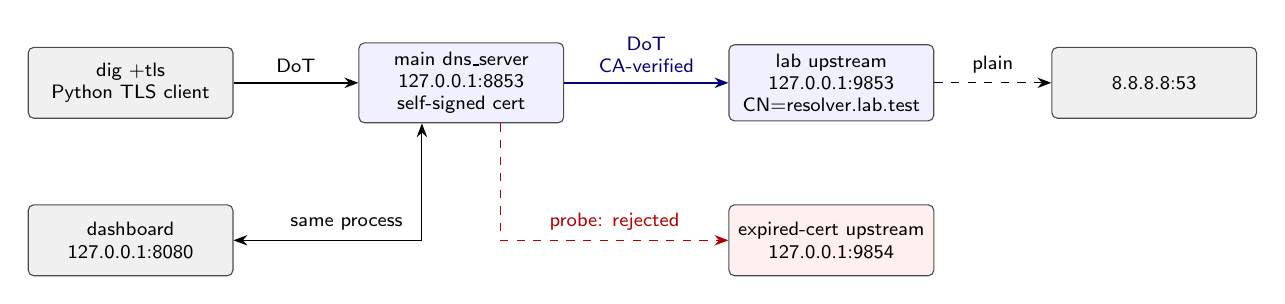
\begin{tikzpicture}[font=\sffamily\scriptsize, >={Stealth[length=5pt]},
  n/.style={draw=black!70, rounded corners=2pt, align=center, minimum height=0.9cm, minimum width=2.6cm, fill=white},
  lab/.style={font=\sffamily\scriptsize}]
\node[n, fill=black!6] (c) at (0,0)    {dig +tls\\Python TLS client};
\node[n, fill=blue!6]  (m) at (4.2,0)  {main dns\_server\\127.0.0.1:8853\\self-signed cert};
\node[n, fill=blue!6]  (u) at (8.9,0)  {lab upstream\\127.0.0.1:9853\\CN=resolver.lab.test};
\node[n, fill=black!6] (g) at (13.0,0) {8.8.8.8:53};
\node[n, fill=black!6] (b) at (0,-2.0)   {dashboard\\127.0.0.1:8080};
\node[n, fill=red!6]   (e) at (8.9,-2.0) {expired-cert upstream\\127.0.0.1:9854};
\draw[->, thick] (c) -- node[lab, above] {DoT} (m);
\draw[->, thick, blue!50!black] (m) -- node[lab, above, align=center] {DoT\\CA-verified} (u);
\draw[->, dashed] (u) -- node[lab, above] {plain} (g);
\draw[<->] (b.east) -| node[lab, above, pos=0.3] {same process} ($(m.south)+(-0.5,0)$);
\draw[->, dashed, red!70!black] ($(m.south)+(0.5,0)$) |- node[lab, above, pos=0.75] {probe: rejected} (e.west);
\end{tikzpicture}
\caption{Lab topology used for the live evaluation. The configured upstream is
\code{tls://127.0.0.1:9853\#resolver.lab.test} with \code{upstream\_ca\_file} pointing at the lab CA.}
\label{fig:lab}
\end{figure}

\subsection{Automated test suite}
\begin{table}[H]
\centering\small
\caption{Automated tests: 534 cases in 54 suites, 31 files. All pass in every build.}\label{tab:suite}
\begin{tabularx}{\textwidth}{@{}LP{4.6cm}P{1.6cm}@{}}
\toprule
Build & Result & Time \\
\midrule
Release build & \passed{}: 534/534 & 13.4 s \\
AddressSanitizer + UndefinedBehaviorSanitizer & \passed{}: 534/534, 0 reports & 27.4 s \\
ThreadSanitizer & \passed{}: 534/534, 0 reports & 15.4 s \\
\bottomrule
\end{tabularx}
\vspace{4pt}
\begin{tabularx}{\textwidth}{@{}P{4.2cm}LP{1.1cm}@{}}
\toprule
Area & Representative suites & Tests \\
\midrule
Wire format, input safety & DnsMessageParse/Encode/Upstream, DomainName, DotFramer, DotFrame, IP, Records & 128 \\
Front end over real TLS & DotServer, TlsContext, Admission & 37 \\
Middleware & Middleware, Responder, DeadlineTimer, InFlightTable, Worker, LoadBalancer, RateLimiter, BlockList, BoundedQueue, Metrics, QueryLog & 97 \\
Upstream DoT, certificates & DotUpstream (24), TlsClient (4), AdminTlsTest (4), MakeFactory (12), ParseUpstream (10) & 54 \\
Resolvers, cache, zones & ForwardingResolver (14), RecursiveResolver, Cache, ZoneFile, ZoneFilesResolver, HostsFile, FindRecords, StubResolver & 161 \\
Config, admin, misc. & ParseConfig, ParseListen, LoadConfig, AdminServerTest, AdminAbuseTest, small type tests & 57 \\
\bottomrule
\end{tabularx}
\end{table}

The upstream tests run against a \textbf{fake DoT server} whose certificate is issued on the fly by a
throw-away test CA with any names, IPs and dates. Each rejection test also asserts that the fake server
\emph{received zero queries}: the question is never sent before the certificate passes.

\subsection{Test cases: expected versus actual}
{\small
\begin{longtable}{@{}P{0.8cm}P{4.4cm}P{3.9cm}P{4.5cm}P{0.9cm}@{}}
\caption{Key test cases (U = unit/integration test, L = live run on the lab topology or, where stated, a phone hotspot). Evidence in the figures
and listings below.}\label{tab:cases}\\
\toprule
Type & Case & Expected & Actual & Result \\
\midrule
\endfirsthead
\toprule
Type & Case & Expected & Actual & Result \\
\midrule
\endhead
\multicolumn{5}{@{}l}{\textit{Normal}}\\
L & \code{dig +tls example.com A} & NOERROR over DoT, upstream over DoT & NOERROR, 2 A records, 11 ms; served by \code{upstream 127.0.0.1:9853 (resolver.lab.test) over TLS} (Lst.~\ref{lst:dig}, Fig.~\ref{fig:lookup}) & \passed \\
L & Same name again & Answer from cache & 0.09 ms, ``cache: hit'' (Fig.~\ref{fig:lookup}) & \passed \\
L & \code{nas.lan}, \code{homeassistant.lan AAAA} & Local records, never forwarded & 192.168.1.20 / fd00::30 from ``records file'' & \passed \\
L & \code{nonexistent-zzq.\allowbreak example.com} & NXDOMAIN passed on & NXDOMAIN & \passed \\
U & \textsf{Dot\allowbreak Upstream.\allowbreak Answers\allowbreak Over\allowbreak Tls\allowbreak With\allowbreak AVerified\allowbreak Certificate} & Answer; SNI sent; subject/issuer recorded & As expected & \passed \\
U & \textsf{Dot\allowbreak Upstream.\allowbreak Connection\allowbreak Is\allowbreak Kept\allowbreak For\allowbreak The\allowbreak Next\allowbreak Query} & Second query reuses the verified connection & 1 handshake, 2 queries & \passed \\
U & \textsf{Dot\allowbreak Upstream.\allowbreak Queries\allowbreak Are\allowbreak Padded}; \textsf{Padded\allowbreak Queries\allowbreak All\allowbreak Have\allowbreak The\allowbreak Block\allowbreak Size} & Every DoT upstream query carries the Padding option; 4- and 60-character names both encode to 128 B & As expected; plain UDP queries stay unpadded & \passed \\
L & Capture of the upstream hop & Upstream records the same size for every name & Queries 147 B, answers 487 B for all four names (Lst.~\ref{lst:pcap}) & \passed \\
\multicolumn{5}{@{}l}{\textit{Upstream certificate validation (negative)}}\\
L+U & Wrong name: lab server checked as \code{dns.google} & Rejected, nothing sent & ``hostname mismatch'' (Fig.~\ref{fig:certs}) & \passed \\
L+U & Expired certificate (9854) & Rejected & ``certificate has expired'' & \passed \\
L+U & Self-signed (our own 8853) & Rejected & ``self-signed certificate'' & \passed \\
L+U & No name, IP not in certificate & Rejected & ``IP address mismatch'' & \passed \\
U & Untrusted issuer; not yet valid; wildcard \code{*.x} for \code{x}; system store vs.\ test CA & Rejected, zero queries received & All rejected, 0 queries & \passed \\
U & \textsf{Make\allowbreak Factory.\allowbreak Tls\allowbreak Upstream\allowbreak With\allowbreak The\allowbreak Wrong\allowbreak Name\allowbreak Fails} & SERVFAIL; \code{rejected = 1}; \code{upstream.queries() = 0} & As expected & \passed \\
U & \textsf{Moves\allowbreak On\allowbreak To\allowbreak The\allowbreak Next\allowbreak Upstream\allowbreak When\allowbreak ACertificate\allowbreak Is\allowbreak Rejected} & Second upstream answers & NOERROR from the second & \passed \\
U & \textsf{AConnection\allowbreak Is\allowbreak Only\allowbreak Reused\allowbreak For\allowbreak The\allowbreak Same\allowbreak Name} & New handshake for another name & New handshake & \passed \\
\multicolumn{5}{@{}l}{\textit{Invalid upstream responses}}\\
U & Garbage reply (TLS) & SERVFAIL, connection dropped & SERVFAIL & \passed \\
U & Reply to another question (wrong ID) & Ignored, SERVFAIL & SERVFAIL & \passed \\
U & Truncated reply; reply cut short mid-frame & SERVFAIL & SERVFAIL & \passed \\
U & \textsf{AFailed\allowbreak Query\allowbreak Does\allowbreak Not\allowbreak Poison\allowbreak The\allowbreak Next\allowbreak One} & Next query succeeds on a fresh connection & NOERROR & \passed \\
U & Junk datagrams before the real answer (UDP) & Junk ignored, real answer used & NOERROR & \passed \\
U & \textsf{Caches\allowbreak Only\allowbreak The\allowbreak Questions\allowbreak Own\allowbreak Chain} & Unrelated records not cached & Not cached & \passed \\
\multicolumn{5}{@{}l}{\textit{Upstream failure and timeouts}}\\
L & Resolver switched to Cloudflare DoT (853 filtered) & SERVFAIL within deadline & SERVFAIL at 1000 ms (per-upstream budget) (Lst.~\ref{lst:fail}) & \passed \\
L & Lab upstream process killed & Fast SERVFAIL & SERVFAIL in 0--1 ms (connection refused) & \passed \\
L & Lab upstream restarted (recovery) & Service resumes, no restart of main & NOERROR 13 ms, 74 ms & \passed \\
U & SilentServerTimesOut (DoT) & SERVFAIL within deadline & SERVFAIL & \passed \\
U & \textsf{Plain\allowbreak Dns\allowbreak Server\allowbreak Is\allowbreak AFailure\allowbreak Not\allowbreak AFallback} & Fails; no plain query sent & 0 plain queries & \passed \\
U & \textsf{Server\allowbreak Closing\allowbreak AKept\allowbreak Connection\allowbreak Is\allowbreak Not\allowbreak An\allowbreak Error} & Transparent reconnect & NOERROR & \passed \\
L & Compare: 8 resolvers on the filtered network & Unreachable ones fail in bounded time & 1.5 s / 3.0 s / 5.0 s SERVFAIL; none hangs (Fig.~\ref{fig:compare}) & \passed \\
L & Public DoT upstreams on a hotspot (Cloudflare, Google, Quad9; system CA store) & Trusted; answers over TLS; wrong name rejected & NOERROR over TLS; \code{1.1.1.1\#dns.google} rejected, hostname mismatch (Lst.~\ref{lst:public}) & \passed \\
\multicolumn{5}{@{}l}{\textit{Adversarial client input (Lst.~\ref{lst:neg})}}\\
L & QDCOUNT=2; label past end; compression loop; space in label & FORMERR & FORMERR & \passed \\
L & Header shorter than 12 bytes; QR=1; zero-length frame & Close, no reply & Closed & \passed \\
L & Opcode STATUS; class CHAOS; type AXFR & NOTIMP & NOTIMP & \passed \\
L & TLS 1.2 client & Handshake refused & Alert 70 ``protocol version'' & \passed \\
L & Abusive client 2{,}000 q/s & Rate limited, then blocked & Blocked after 0.09 s; 15{,}831 refused (Fig.~\ref{fig:abuse}) & \passed \\
L & Polite client 50 q/s & Never refused & 400/400 answered & \passed \\
\multicolumn{5}{@{}l}{\textit{Load and failure recovery}}\\
L & load\_gen 100k flood; 20\% failures; overload & Exactly one reply per query (exit 0) & exit 0 in all three runs & \passed \\
L & Failures test: 60\% injected, then 0\% & Breakers open, then close & All 4 open (7 trips each), all closed after (Fig.~\ref{fig:breakers}) & \passed \\
\bottomrule
\end{longtable}
}

\subsection{Evidence: a DNS query completing over DNS-over-TLS}\label{sec:ev-dot}

\begin{lstlisting}[caption={\code{dig +tls} through the full chain (client DoT $\rightarrow$ server $\rightarrow$ DoT to the verified lab upstream)},label={lst:dig}]
$ dig +tls @127.0.0.1 -p 8853 example.com A
;; ->>HEADER<<- opcode: QUERY, status: NOERROR, id: 5923
;; flags: qr rd ra; QUERY: 1, ANSWER: 2, AUTHORITY: 0, ADDITIONAL: 1
; EDNS: version: 0, flags:; udp: 1232
;; ANSWER SECTION:
example.com.            66      IN      A       172.66.147.243
example.com.            66      IN      A       104.20.23.154
;; Query time: 11 msec
;; SERVER: 127.0.0.1#8853(127.0.0.1) (TLS)
\end{lstlisting}

\begin{figure}[H]
\centering
% \subcaptionbox bottom-aligns the images and top-aligns the captions,
% so (a), (b) and (c) start on the same line despite different heights.
\subcaptionbox{First lookup: miss, served by the DoT upstream.}[0.32\textwidth]{%
  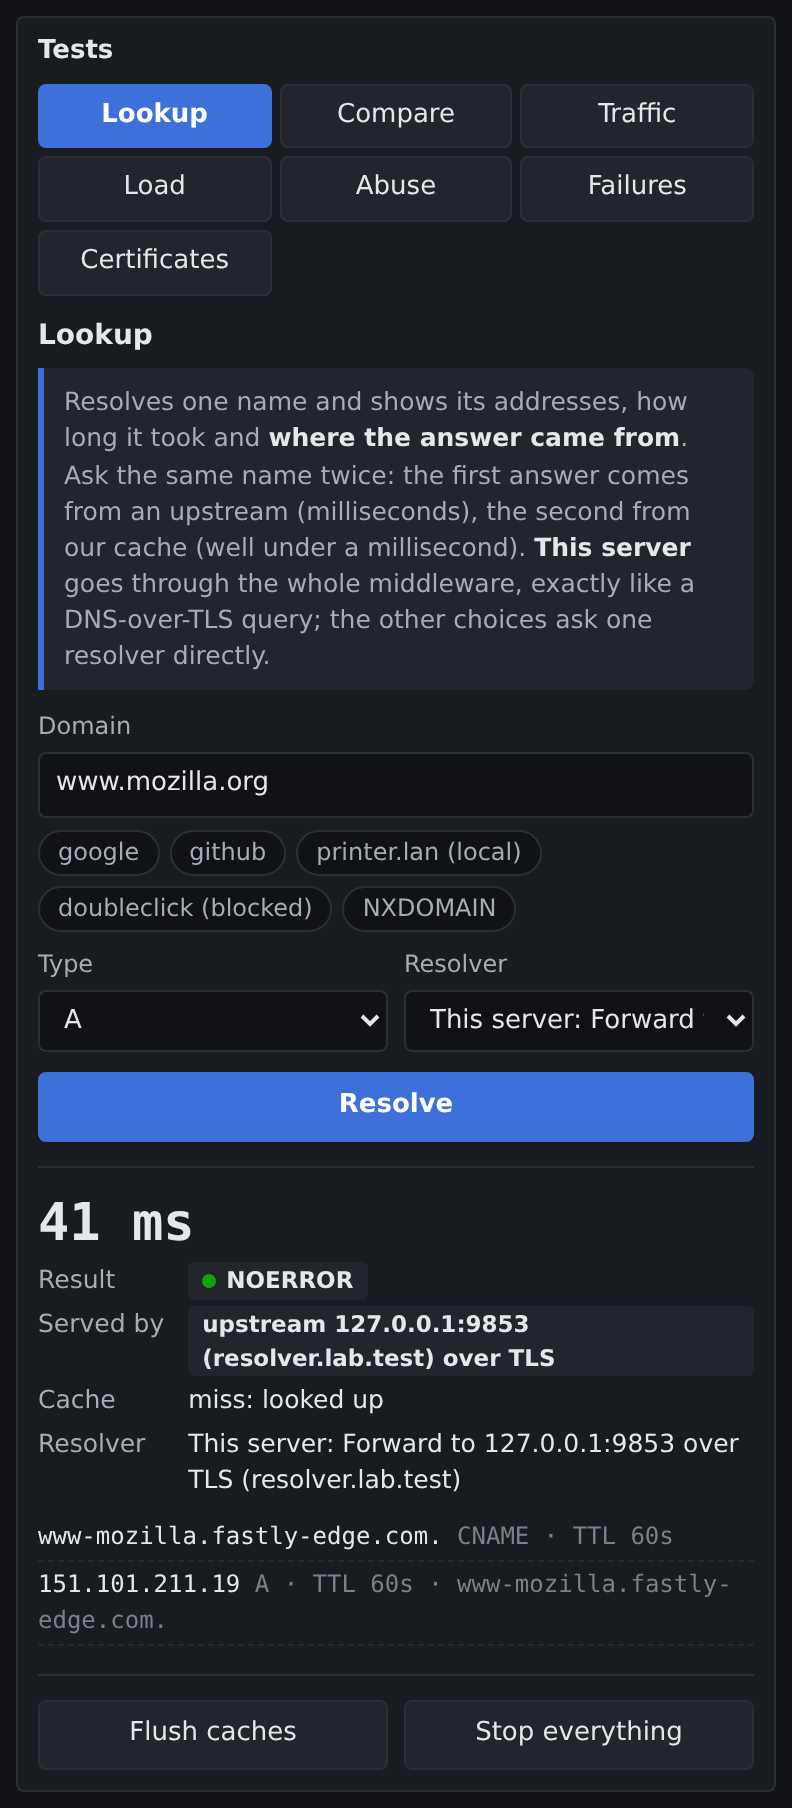
\includegraphics[width=0.32\textwidth]{lookup_tls_cold.png}}\hfill
\subcaptionbox{Second lookup: cache hit, 0.09 ms.}[0.32\textwidth]{%
  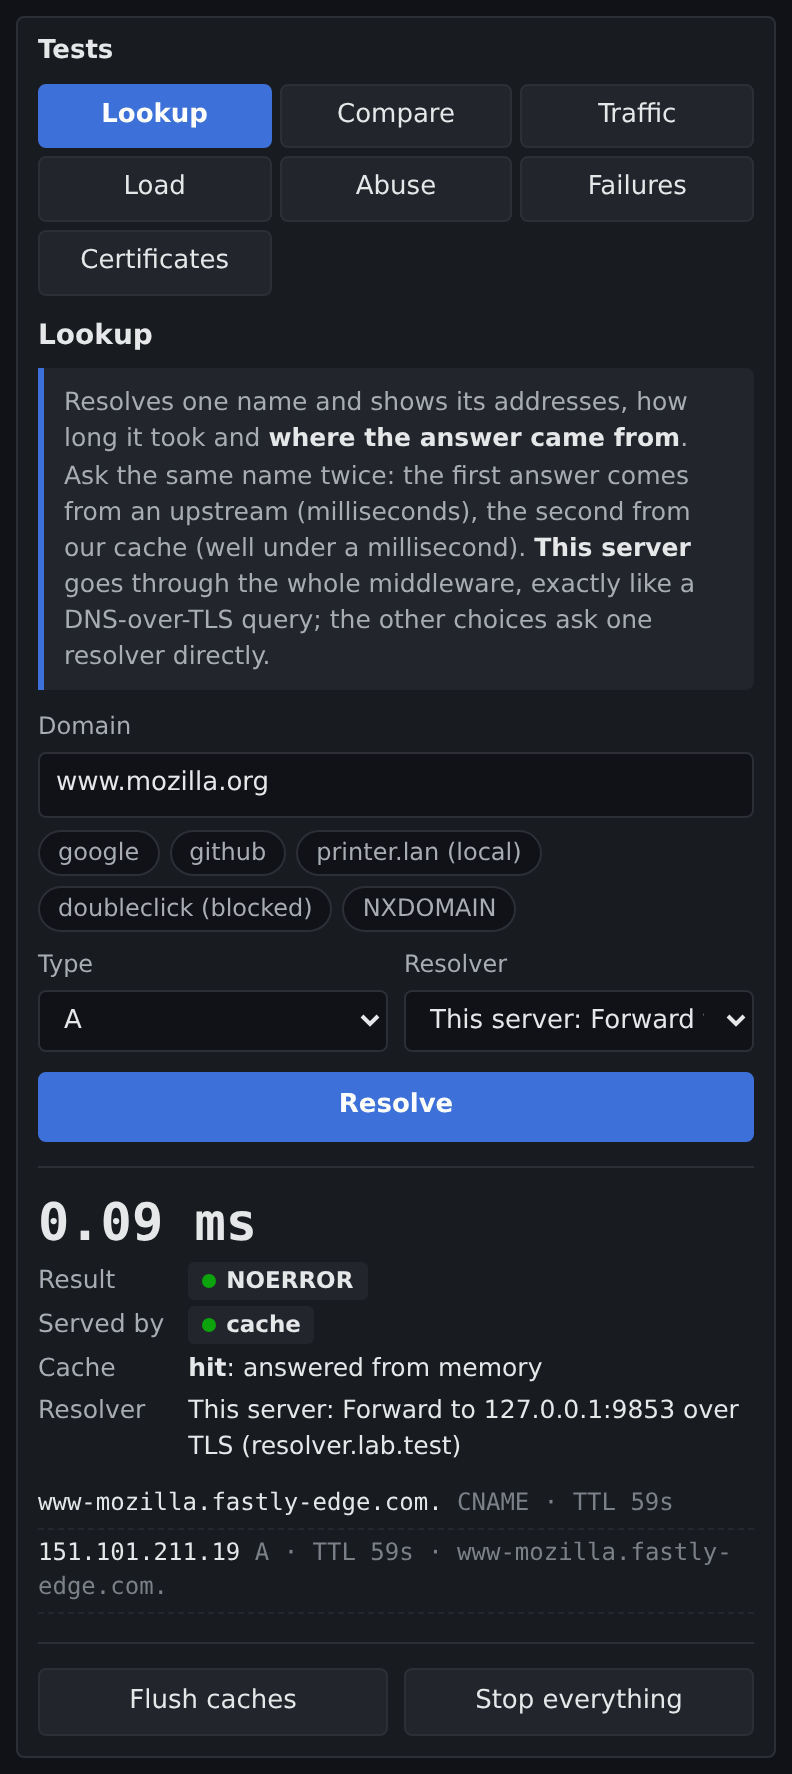
\includegraphics[width=0.32\textwidth]{lookup_tls_cached.png}}\hfill
\subcaptionbox{Local record, blocked domain (REFUSED) and NXDOMAIN.}[0.32\textwidth]{%
  \begin{minipage}[b]{0.32\textwidth}
  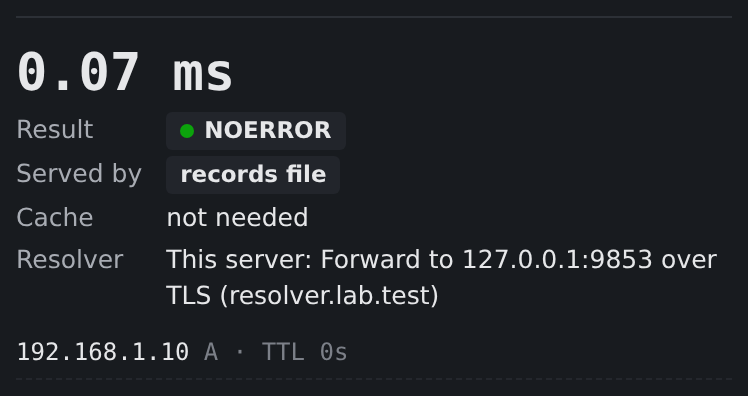
\includegraphics[width=\linewidth]{lookup_local.png}\\[3pt]
  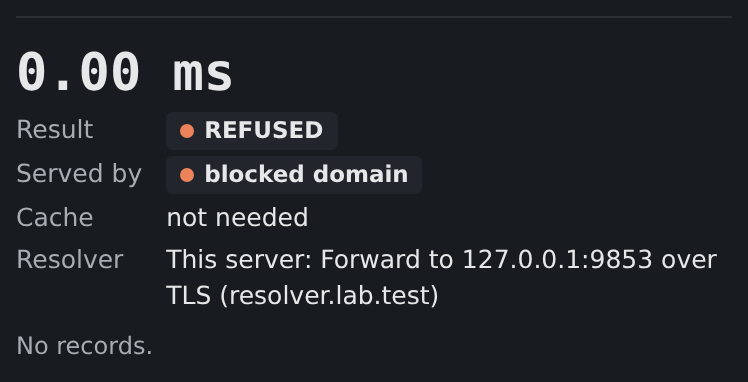
\includegraphics[width=\linewidth]{lookup_blocked.png}\\[3pt]
  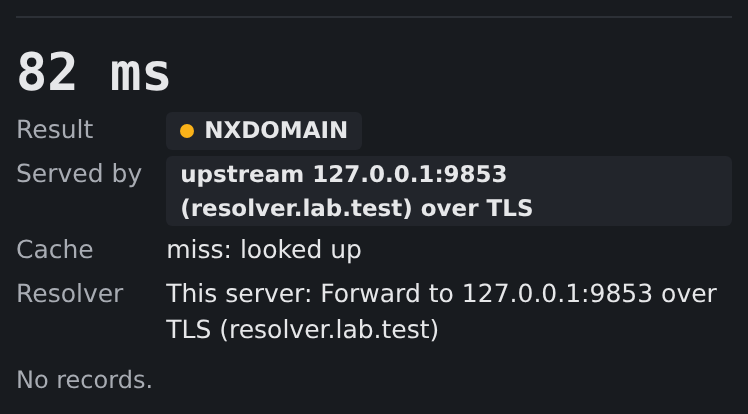
\includegraphics[width=\linewidth]{lookup_nx.png}
  \end{minipage}}
\caption{Dashboard Lookup test. ``This server'' sends the query through the whole middleware, like a DoT
client. ``Served by'' names the hop that answered: \code{upstream 127.0.0.1:9853 (resolver.lab.test) over TLS}.}
\label{fig:lookup}
\end{figure}

\needspace{12\baselineskip}
\textbf{Packet capture of both hops.} 83 packets were captured on the isolated loopback: four client
connections to :8853 and one upstream connection to :9853, reused for all four names.
\begin{lstlisting}[caption={\code{tshark} on the capture: what an on-path observer sees},label={lst:pcap}]
No.  src->dst      len  info
  4  40037->8853   369  Client Hello                      (ALPN "dot", TLS 1.3)
  6  8853->40037   879  Server Hello, Change Cipher Spec, Application Data x4
  9  8853->40037   321  Application Data
 10  40037->8853   558  Application Data                  query, padded: TLS record 487 B
 15  45352->9853   385  Client Hello                      SNI "resolver.lab.test"  (upstream hop)
 17  9853->45352   905  Server Hello, Change Cipher Spec, Application Data x4
 22  45352->9853   218  Application Data                  upstream query, padded:  TLS record 147 B
 23  9853->45352   558  Application Data                  upstream answer, padded: TLS record 487 B
 24  8853->40037   558  Application Data                  reply, padded: TLS record 487 B
 40  45352->9853   218  Application Data                  2nd name, same upstream connection (reused), 147 B
 41  9853->45352   558  Application Data                  its answer, 487 B
 ...
$ tshark -r dot.pcap -Y dns | wc -l                       ->  0   (no DNS message is readable)
$ strings dot.pcap | grep -ciE 'example|wikipedia|longer-name' ->  0   (no queried name appears)
TLS record sizes by name             client hop reply   upstream query   upstream answer
  example.com                               487 B            147 B             487 B
  www.wikipedia.org                         487 B            147 B             487 B
  a-much-longer-name-...example.org         487 B            147 B             487 B
  example.com, client asked no padding       86 B            147 B             487 B
\end{lstlisting}

\needspace{11\baselineskip}
\begin{lstlisting}[caption={Client-facing TLS parameters and the server key's protection}]
$ openssl s_client -connect 127.0.0.1:8853 -alpn dot -brief
Protocol version: TLSv1.3        Ciphersuite: TLS_AES_256_GCM_SHA384
Server Temp Key: X25519, 253 bits          (ephemeral ECDHE -> forward secrecy)
$ openssl s_client -connect 127.0.0.1:8853 -tls1_2
... tlsv1 alert protocol version ... SSL alert number 70     (TLS 1.2 refused)
$ ls -l config/server.key ; git check-ignore -v config/server.key
-rw------- 1 xyz xyz 241 config/server.key
.gitignore:7:*.key   config/server.key
\end{lstlisting}

\subsection{Evidence: upstream certificate validation}\label{sec:ev-cert}
\begin{figure}[H]
\centering
\begin{subfigure}[t]{0.33\textwidth}\vspace{0pt}\centering
  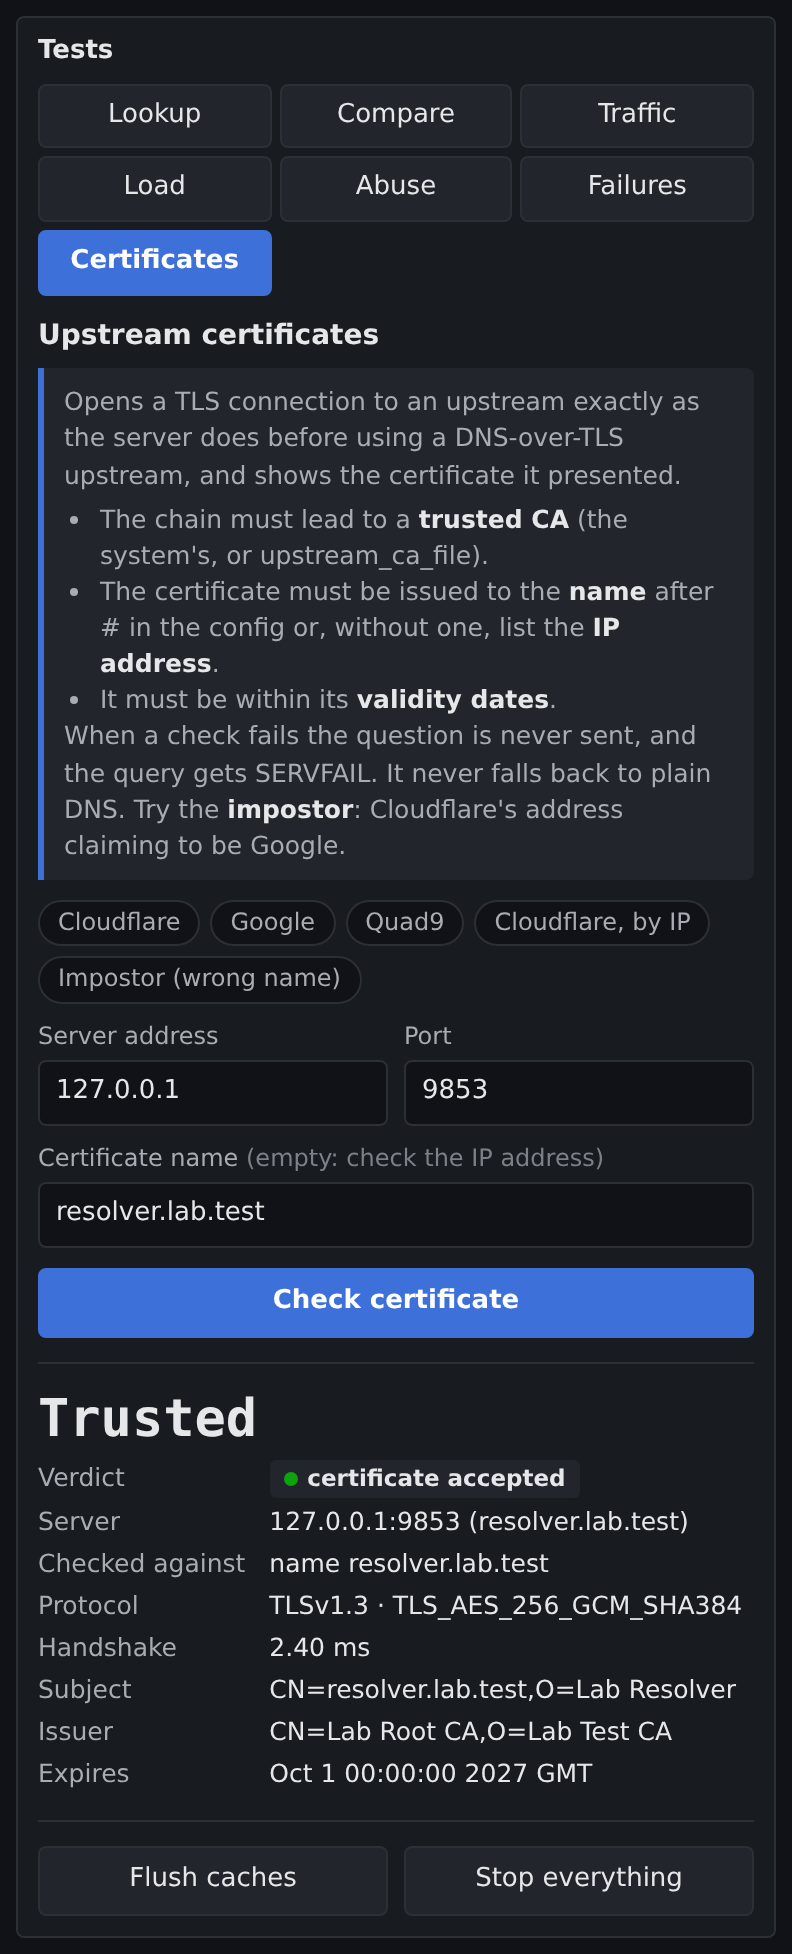
\includegraphics[width=\linewidth]{cert_ok.png}
  \caption{Accepted: chain to the lab CA, name \code{resolver.lab.test}, TLS 1.3.}
\end{subfigure}\hfill
\begin{subfigure}[t]{0.64\textwidth}\vspace{0pt}\centering
  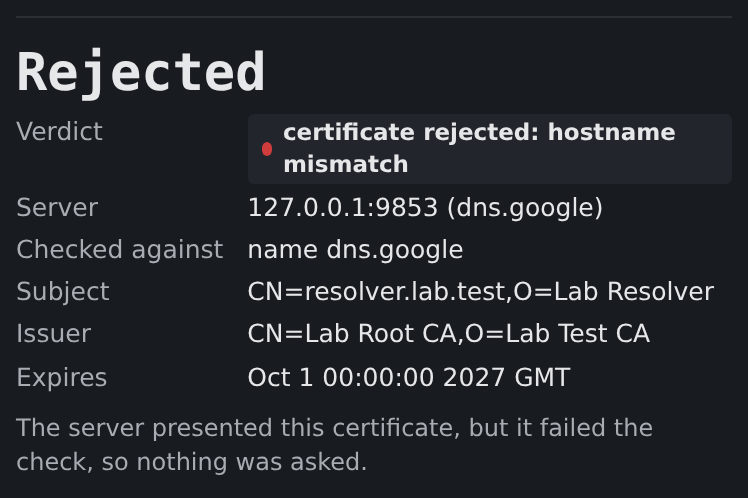
\includegraphics[width=0.49\linewidth]{cert_wrong_name.png}\hfill
  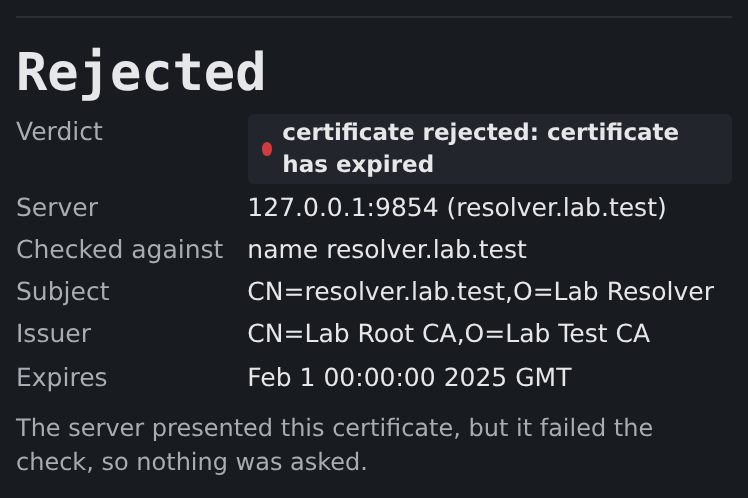
\includegraphics[width=0.49\linewidth]{cert_expired.png}\\[4pt]
  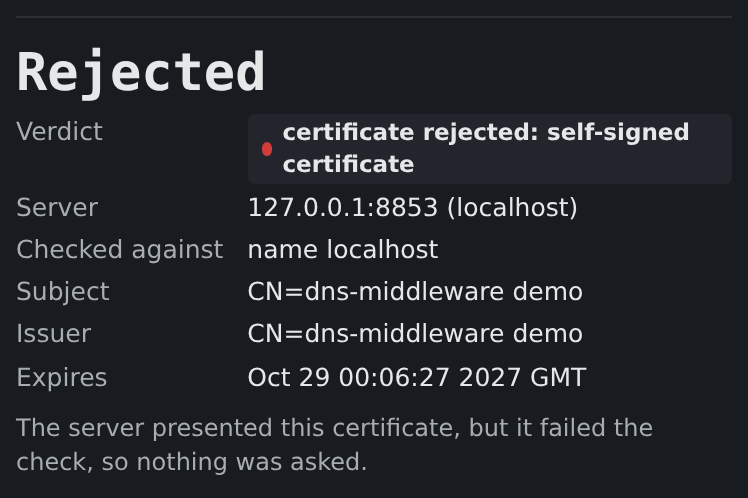
\includegraphics[width=0.49\linewidth]{cert_self_signed.png}\hfill
  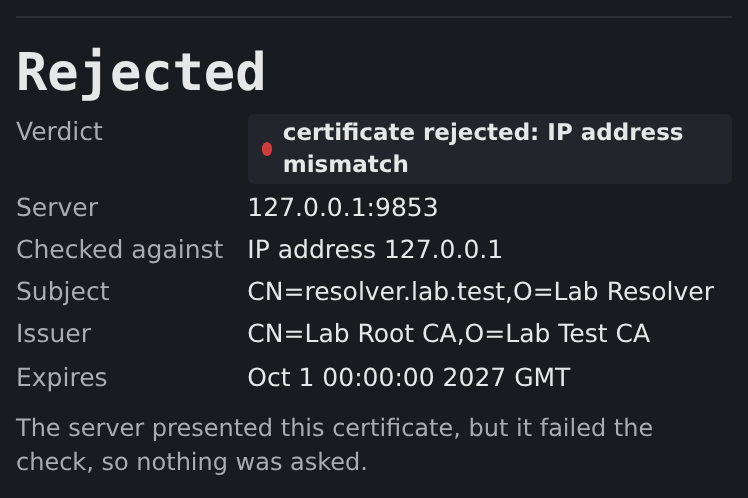
\includegraphics[width=0.49\linewidth]{cert_by_ip.png}\\[4pt]
  \centering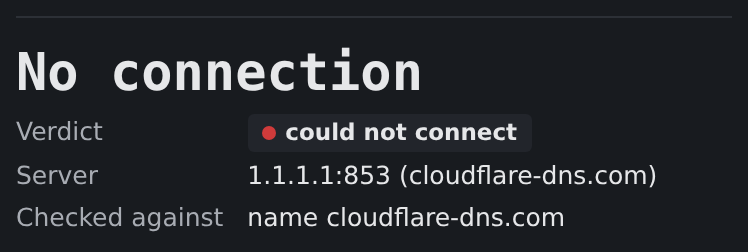
\includegraphics[width=0.49\linewidth]{cert_unreachable.png}
  \caption{Rejected: hostname mismatch (impostor), expired, self-signed, IP address mismatch; and ``could not
  connect'' for Cloudflare on the filtered network. Each says ``nothing was asked''.}
\end{subfigure}
\caption{Dashboard Certificates test: one real handshake per probe, made by the same \code{TlsClient} the
resolver uses.}
\label{fig:certs}
\end{figure}

\begin{figure}[H]
\centering
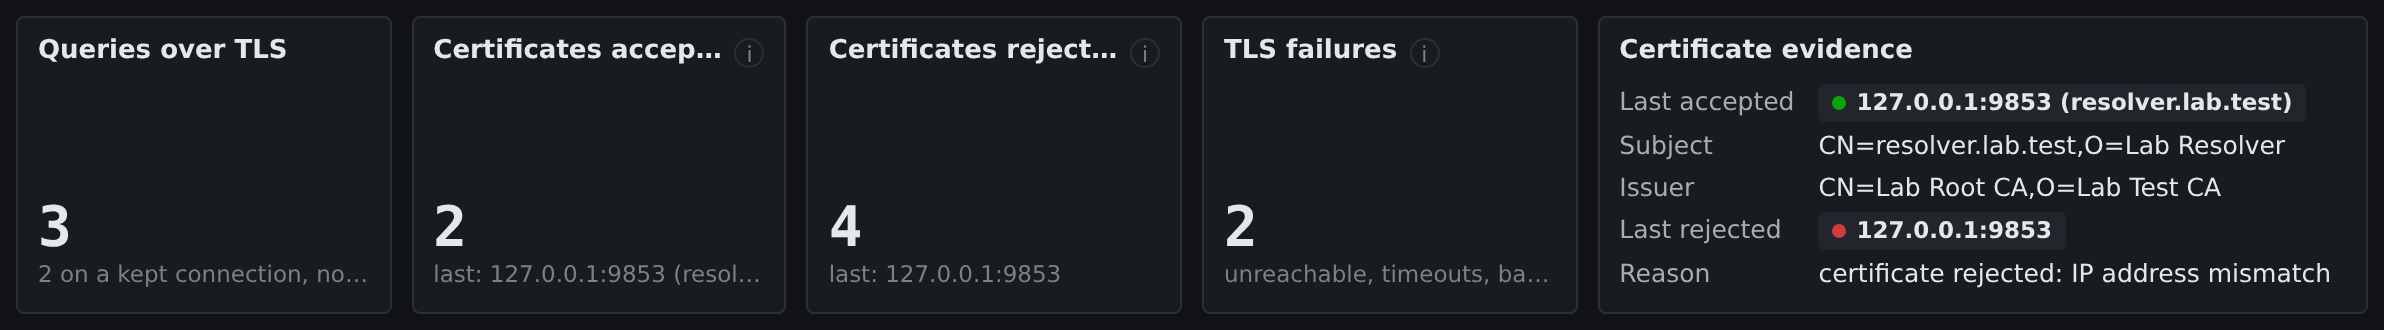
\includegraphics[width=\textwidth]{tls_row.png}
\caption{``Upstream encryption'' row after the probes: queries over TLS (2 of 3 on a kept connection),
certificates accepted and rejected, the accepted certificate's subject and issuer, and the last rejection's
reason.}
\label{fig:tlsrow}
\end{figure}

\needspace{8\baselineskip}
The same checks from the command line, independent of our code:
\begin{lstlisting}
$ openssl s_client -connect 127.0.0.1:9853 -CAfile ca.pem -verify_hostname resolver.lab.test -brief
Protocol version: TLSv1.3   Peer certificate: O = Lab Resolver, CN = resolver.lab.test
Verification: OK            Verified peername: resolver.lab.test
$ openssl s_client -connect 127.0.0.1:9854 -CAfile ca.pem -verify_hostname resolver.lab.test -verify_return_error
verify error:num=10:certificate has expired   notAfter=Feb  1 00:00:00 2025 GMT
\end{lstlisting}

\needspace{14\baselineskip}
On an unfiltered network the public resolvers go through the same code, trusted via the system CA store:
\begin{lstlisting}[caption={Public DoT upstreams on a phone hotspot (\code{config/demo.conf}, system CA store)},label={lst:public}]
$ dig +tls @127.0.0.1 -p 8853 example.com A     status: NOERROR  Query time: 156 msec
$ dig +tls @127.0.0.1 -p 8853 github.com A      status: NOERROR  Query time: 21 msec
$ dig +tls @127.0.0.1 -p 8853 github.com A      status: NOERROR  Query time: 1 msec   (cache)
  served by: upstream 1.1.1.1:853 (cloudflare-dns.com) over TLS
  upstream TLS: 1 handshake, 2 reused, 0 rejected; issuer CN=SSL.com SSL Intermediate CA ECC R2
Certificates test       1.1.1.1#cloudflare-dns.com  -> Trusted, TLSv1.3
                        8.8.8.8#dns.google          -> Trusted, TLSv1.3
                        9.9.9.9#dns.quad9.net       -> Trusted, TLSv1.3
                        1.1.1.1#dns.google          -> certificate rejected: hostname mismatch
Lookup (direct)         Cloudflare, Google, Quad9 over TLS -> NOERROR, "over TLS"
\end{lstlisting}

\subsection{Evidence: invalid responses, upstream failure, timeouts and recovery}
\begin{lstlisting}[caption={Failure and recovery seen by a real DoT client (\code{dig +tls}, one try each)},label={lst:fail}]
## 1. Normal: configured DoT upstream (resolver.lab.test)
github.com           status: NOERROR   Query time: 9 msec
## 2. Timeout: resolver switched to Cloudflare over TLS (port 853 filtered on this network)
github.com           status: SERVFAIL  Query time: 1001 msec
www.mozilla.org      status: SERVFAIL  Query time: 1000 msec
## 3. Back to the configured upstream
github.com           status: NOERROR   Query time: 1 msec
## 4. Upstream failure: the lab DoT upstream process is stopped
www.python.org       status: SERVFAIL  Query time: 0 msec
www.rust-lang.org    status: SERVFAIL  Query time: 1 msec
## 5. Recovery: the upstream is started again (main server untouched)
www.python.org       status: NOERROR   Query time: 13 msec
www.rust-lang.org    status: NOERROR   Query time: 74 msec
\end{lstlisting}

\begin{figure}[H]
\centering
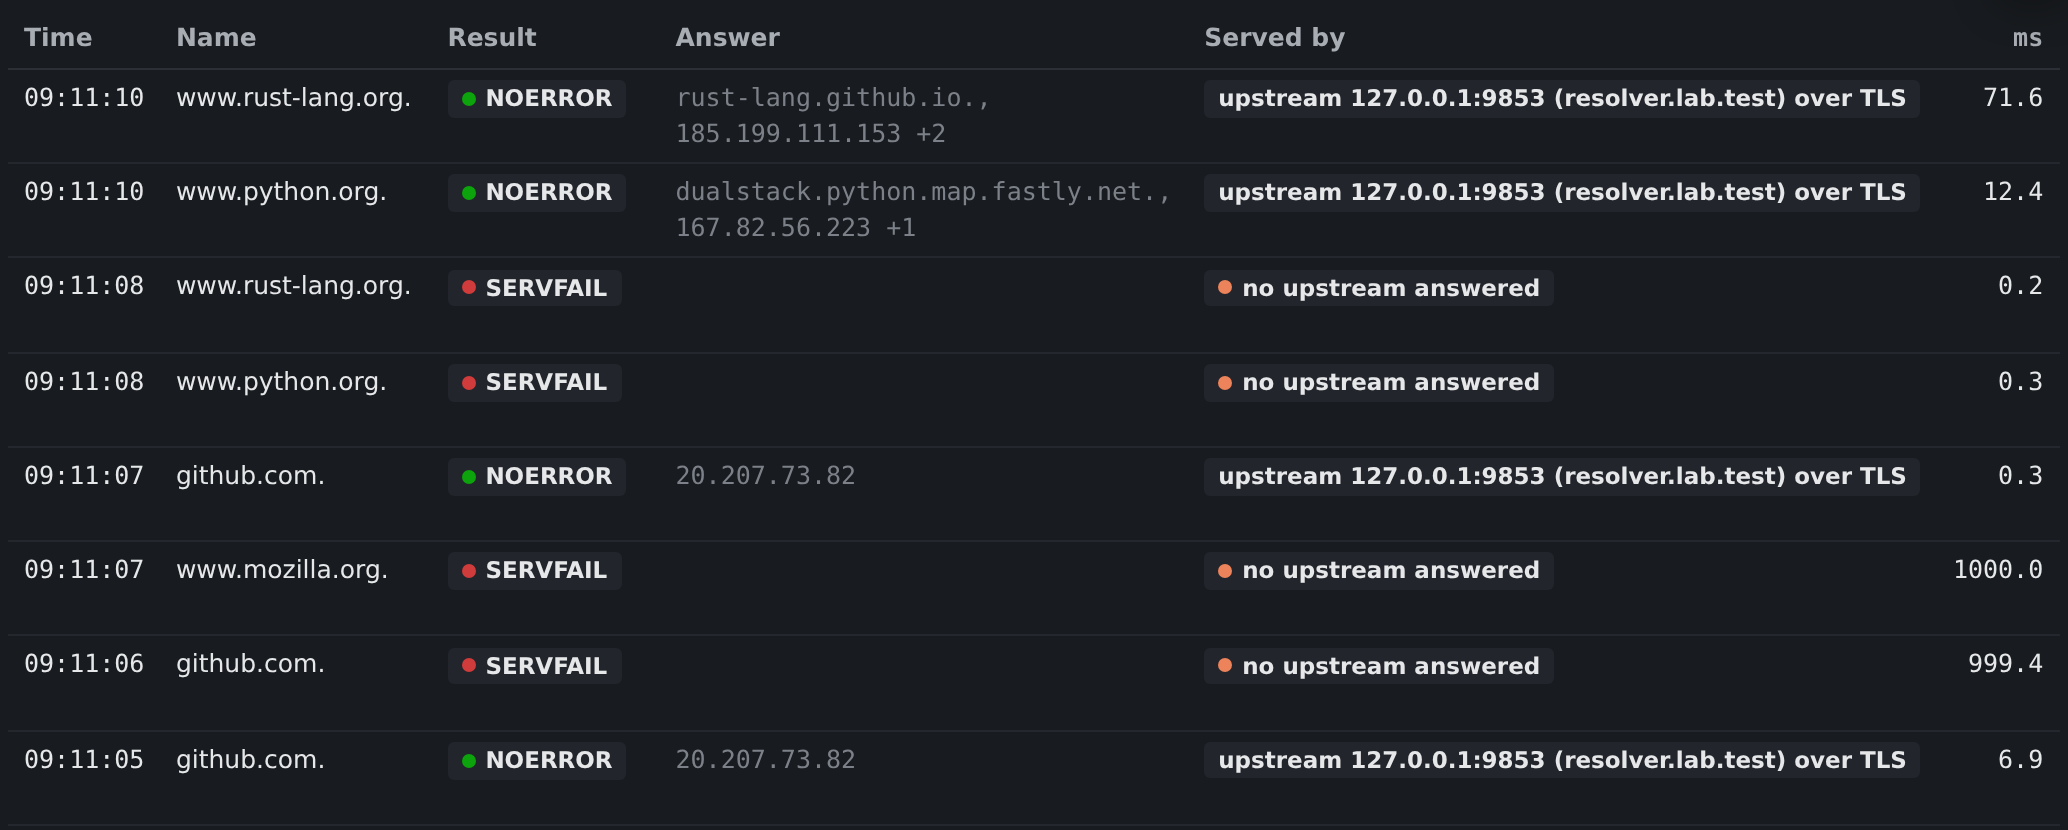
\includegraphics[width=\textwidth]{live_queries_narrow.png}
\caption{Live query log for Listing~\ref{lst:fail}, newest first: success over TLS, SERVFAIL ``no upstream
answered'' at the 1000~ms upstream budget, fast SERVFAIL while the upstream is down, and recovery. The Client
(always 127.0.0.1 over DoT) and Type (always A) columns are cropped out.}
\label{fig:log}
\end{figure}

\begin{figure}[H]
\centering
% one 8-row screenshot split into two halves, header repeated, so it can be shown at a readable size
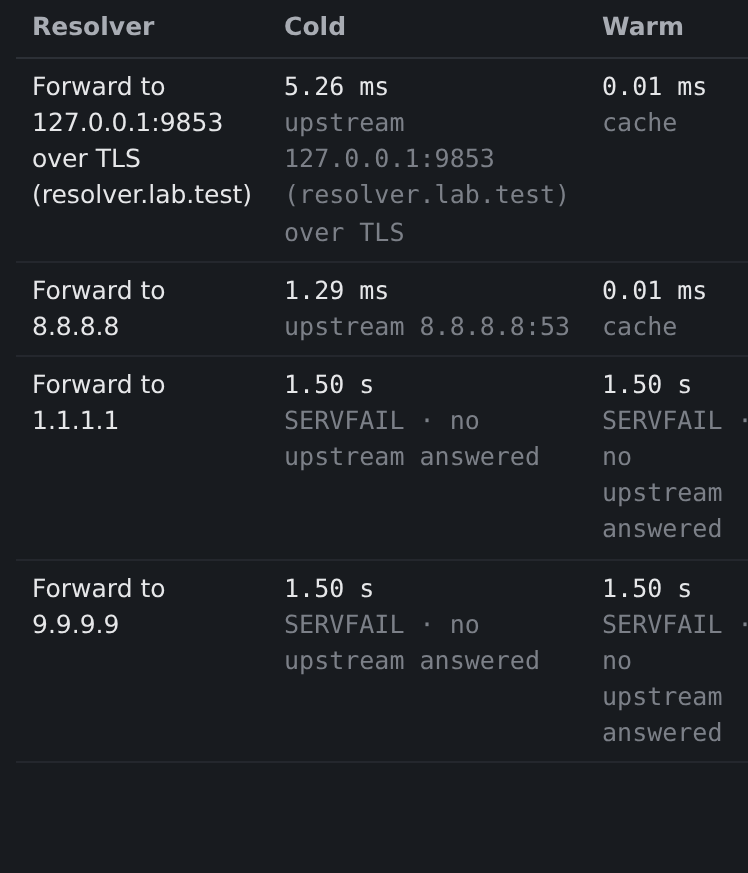
\includegraphics[width=0.48\textwidth]{compare_1.png}\hfill
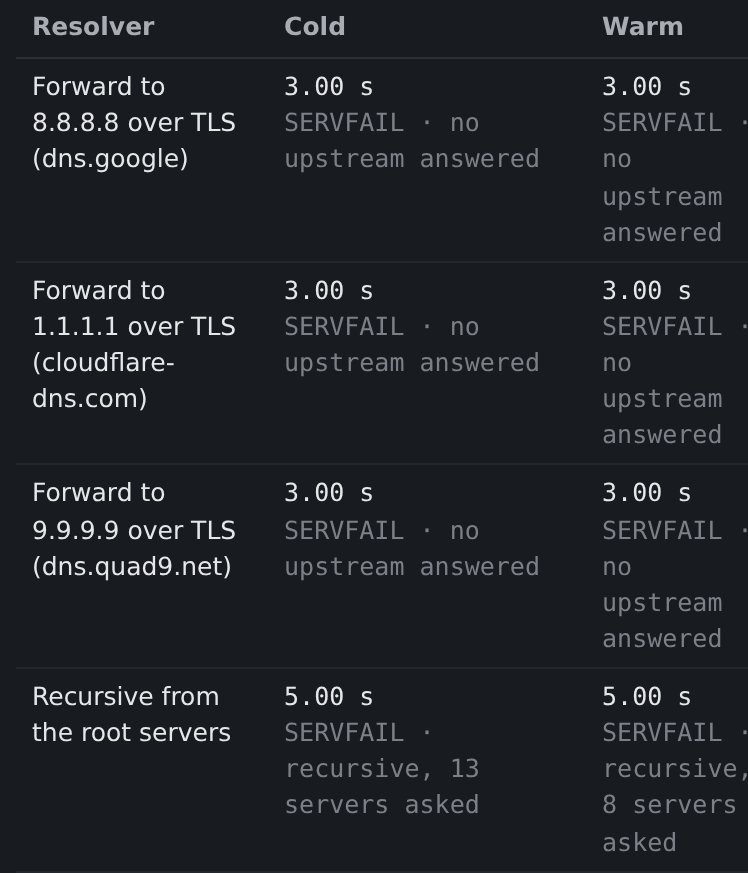
\includegraphics[width=0.48\textwidth]{compare_2.png}
\caption{Compare test on the filtered campus network (rows 1--4 left, 5--8 right). Only the lab DoT upstream
and 8.8.8.8 answer. Every unreachable resolver fails with SERVFAIL in bounded time: plain upstreams 1.5~s, DoT
upstreams 3.0~s, recursion 5.0~s after asking 13 servers within its budget. These are direct calls that bypass
the middleware. Through the middleware the 2~s deadline (or the 1~s per-upstream budget) applies, as
Listing~\ref{lst:fail} shows.}
\label{fig:compare}
\end{figure}

\begin{figure}[H]
\centering
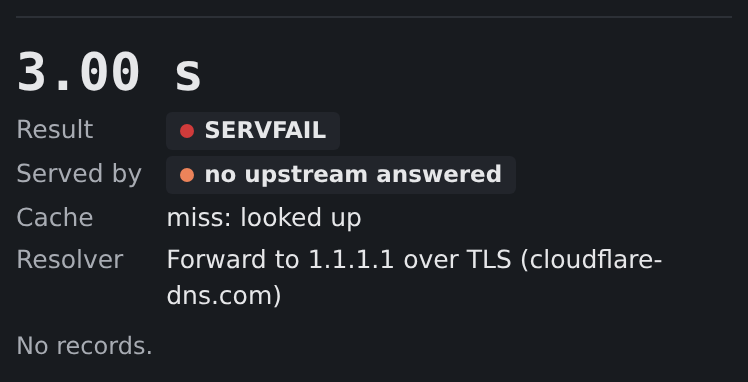
\includegraphics[width=0.5\textwidth]{lookup_unreachable_tls.png}
\caption{Lookup through Cloudflare over TLS on the filtered network: SERVFAIL ``no upstream answered''. It
never falls back to plain DNS.}
\label{fig:unreachable}
\end{figure}

\begin{lstlisting}[caption={Hand-made malformed and unsupported DoT messages (Python \code{ssl} client)},label={lst:neg}]
valid query example.com A                    -> NOERROR (id 0x1234, 83 bytes)
truncated header (5 bytes)                   -> connection closed, no reply
QDCOUNT=2                                    -> FORMERR (id 0x1234, 12 bytes)
label length runs past the end               -> FORMERR (id 0x1234, 12 bytes)
compression pointer loop                     -> FORMERR (id 0x1234, 12 bytes)
bad name syntax (space in label)             -> FORMERR (id 0x1234, 12 bytes)
response bit set (QR=1)                      -> connection closed, no reply
opcode STATUS (2)                            -> NOTIMP (id 0x1234, 12 bytes)
class CHAOS                                  -> NOTIMP (id 0x1234, 12 bytes)
type AXFR (252)                              -> NOTIMP (id 0x1234, 12 bytes)
blocked domain ad.doubleclick.net            -> REFUSED (id 0x1234, 36 bytes)
zero-length frame                            -> connection closed, no reply
\end{lstlisting}

\subsection{Evidence: availability under load and abuse}
\begin{figure}[H]
\centering
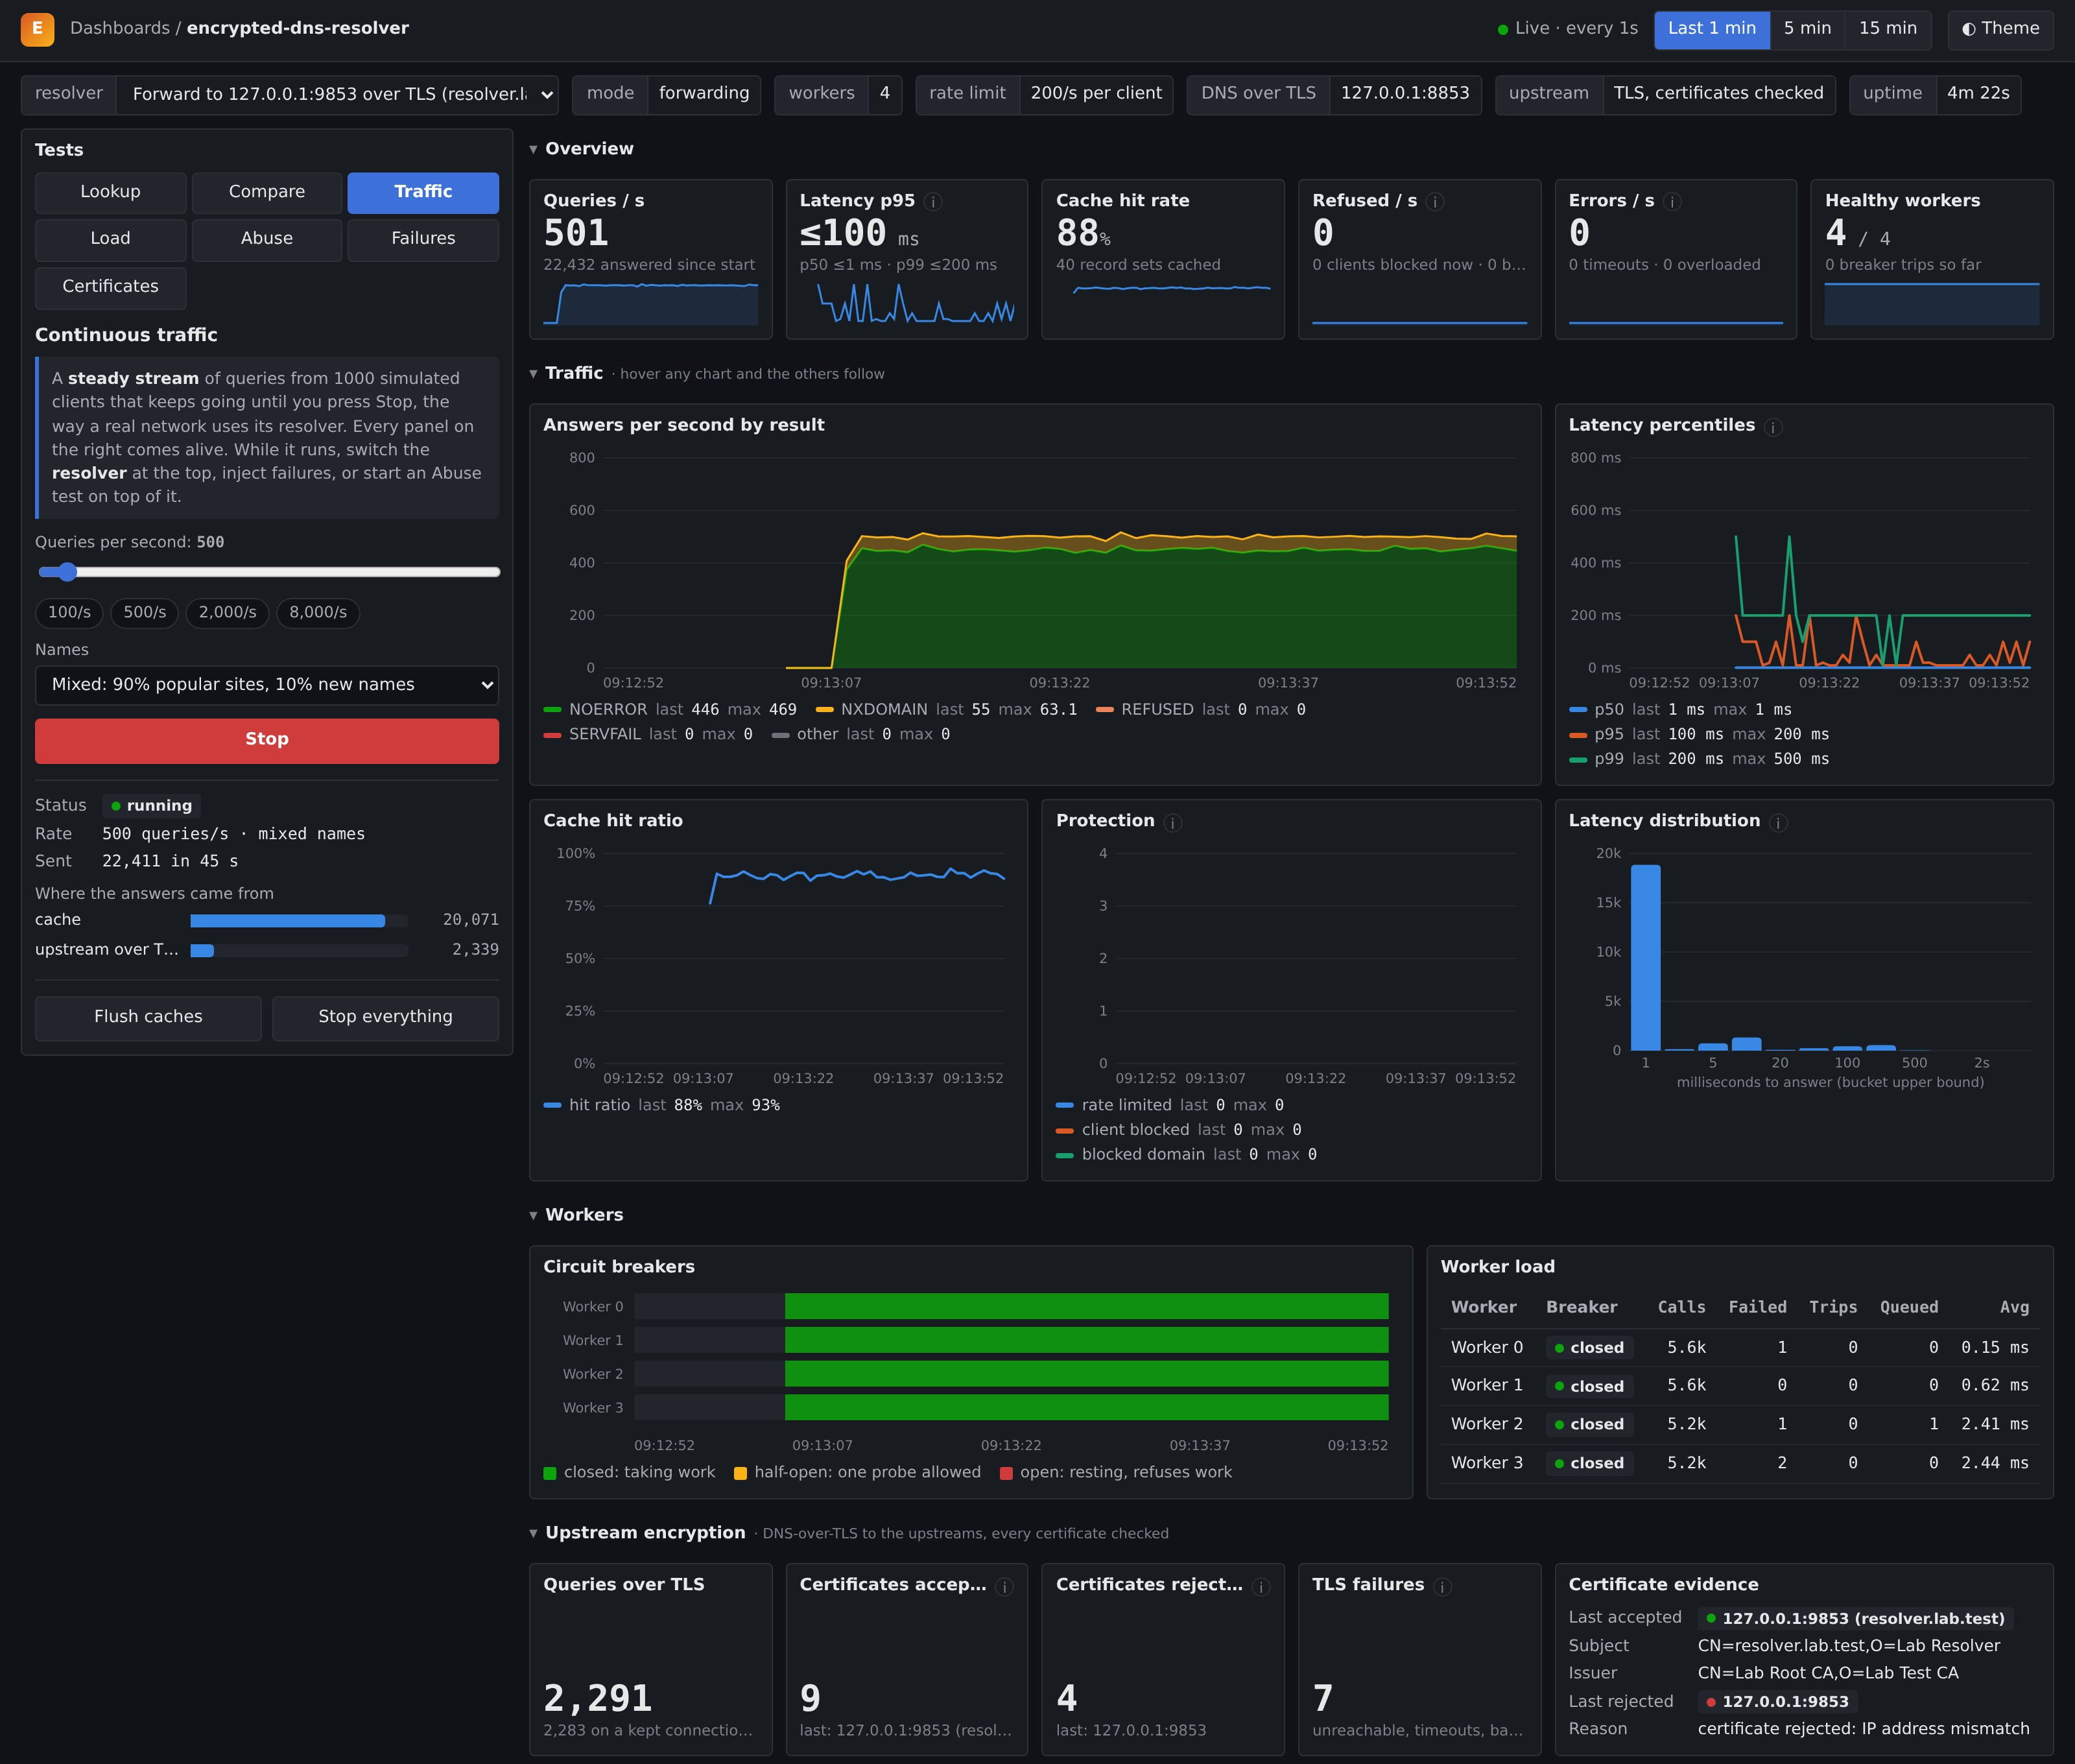
\includegraphics[width=\textwidth]{overview.jpg}
\caption{Dashboard (dark mode) during the Traffic test: 500 q/s from 1000 simulated clients, 90\% popular and
10\% new names, for 45~s. 22{,}432 answered, 0 errors, cache hit rate 88\%, p50 $\le$1~ms, p95 $\le$100~ms;
2{,}339 answers from the DoT upstream, 2{,}283 of them on a kept connection; all four breakers closed.}
\label{fig:overview}
\end{figure}

\begin{figure}[H]
\centering
\begin{subfigure}[b]{0.31\textwidth}\centering
  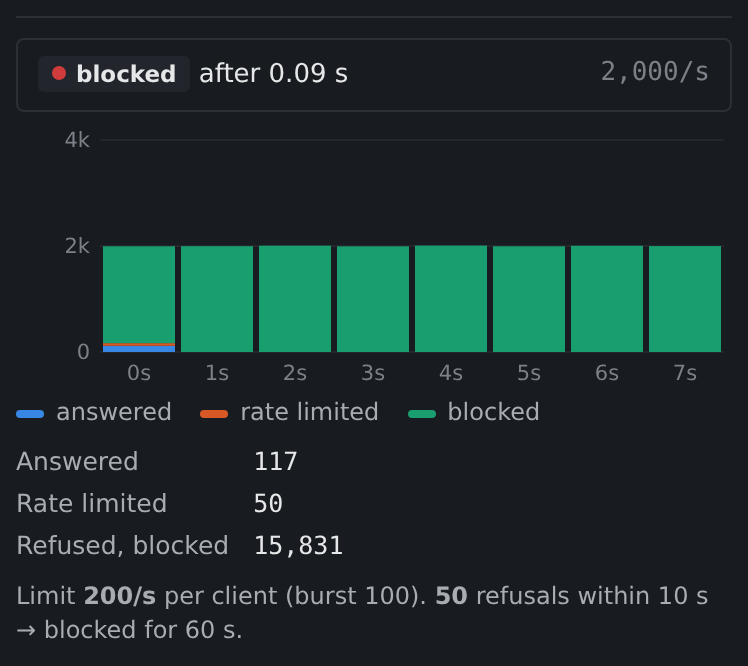
\includegraphics[height=4.4cm]{abuse.png}
  \caption{2{,}000 q/s: blocked after 0.09~s.}
\end{subfigure}\hfill
\begin{subfigure}[b]{0.31\textwidth}\centering
  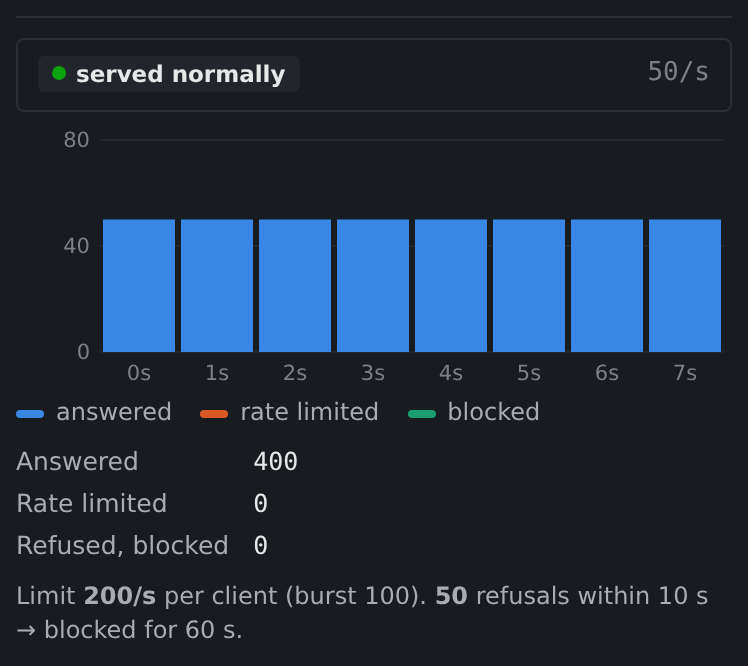
\includegraphics[height=4.4cm]{abuse_polite.png}
  \caption{50 q/s: served normally.}
\end{subfigure}\hfill
\begin{subfigure}[b]{0.33\textwidth}\centering
  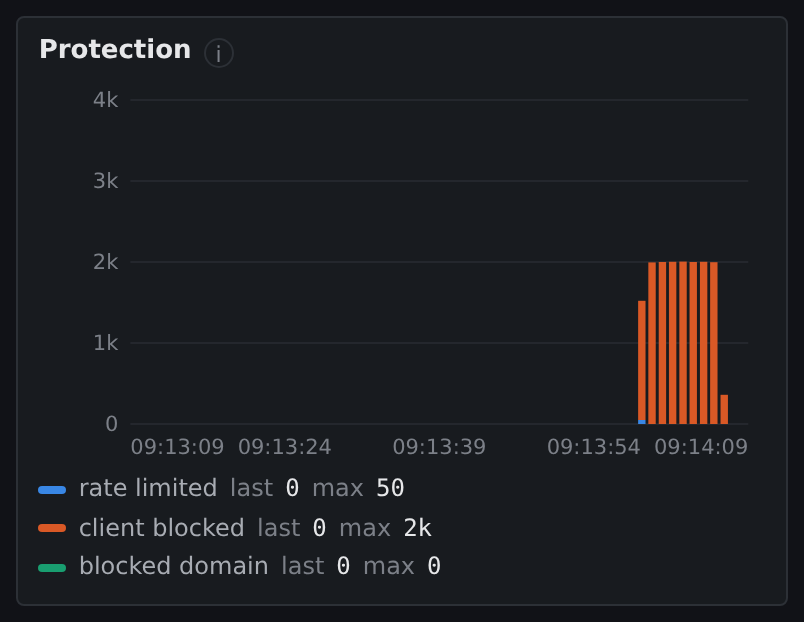
\includegraphics[height=4.4cm]{protection.png}
  \caption{Protection panel: client blocked.}
\end{subfigure}\\[8pt]
\begin{subfigure}[b]{0.55\textwidth}\centering
  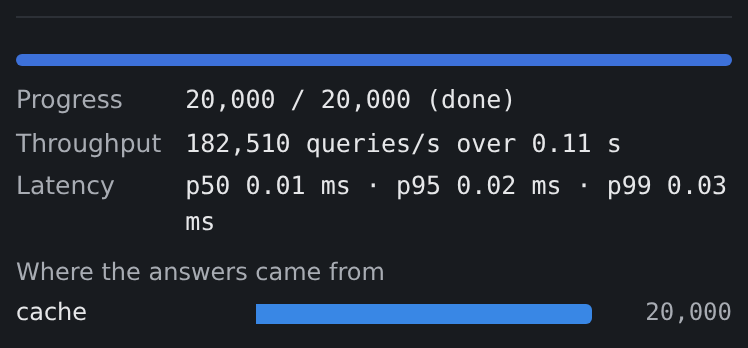
\includegraphics[width=\linewidth]{load.png}
  \caption{Load test: 20k cached queries at 182k q/s.}
\end{subfigure}
\caption{Abuse and Load tests. The abusive client got 117 answers and 50 rate-limited replies, then 15{,}831
REFUSED while blocked. The polite client was never refused.}
\label{fig:abuse}
\end{figure}

\begin{figure}[H]
\centering
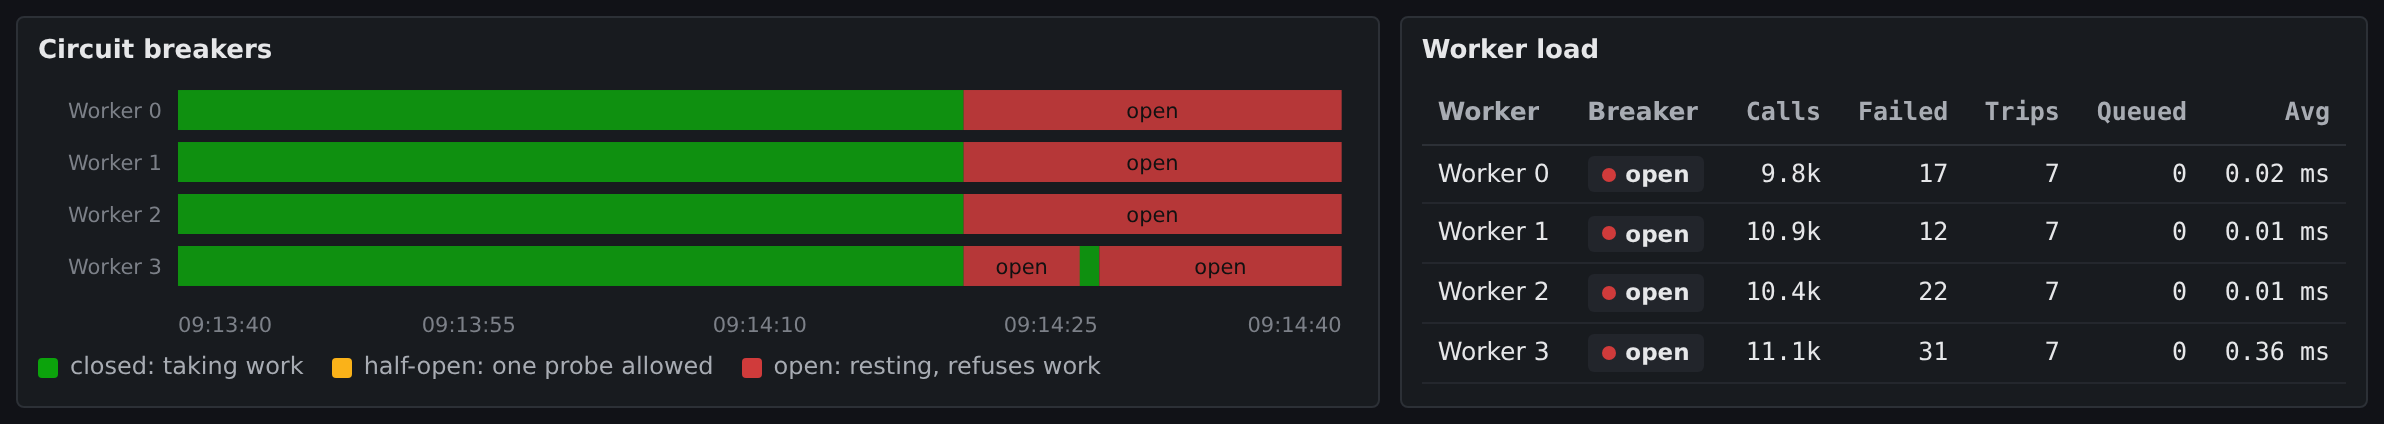
\includegraphics[width=\textwidth]{failures_open.png}\\[4pt]
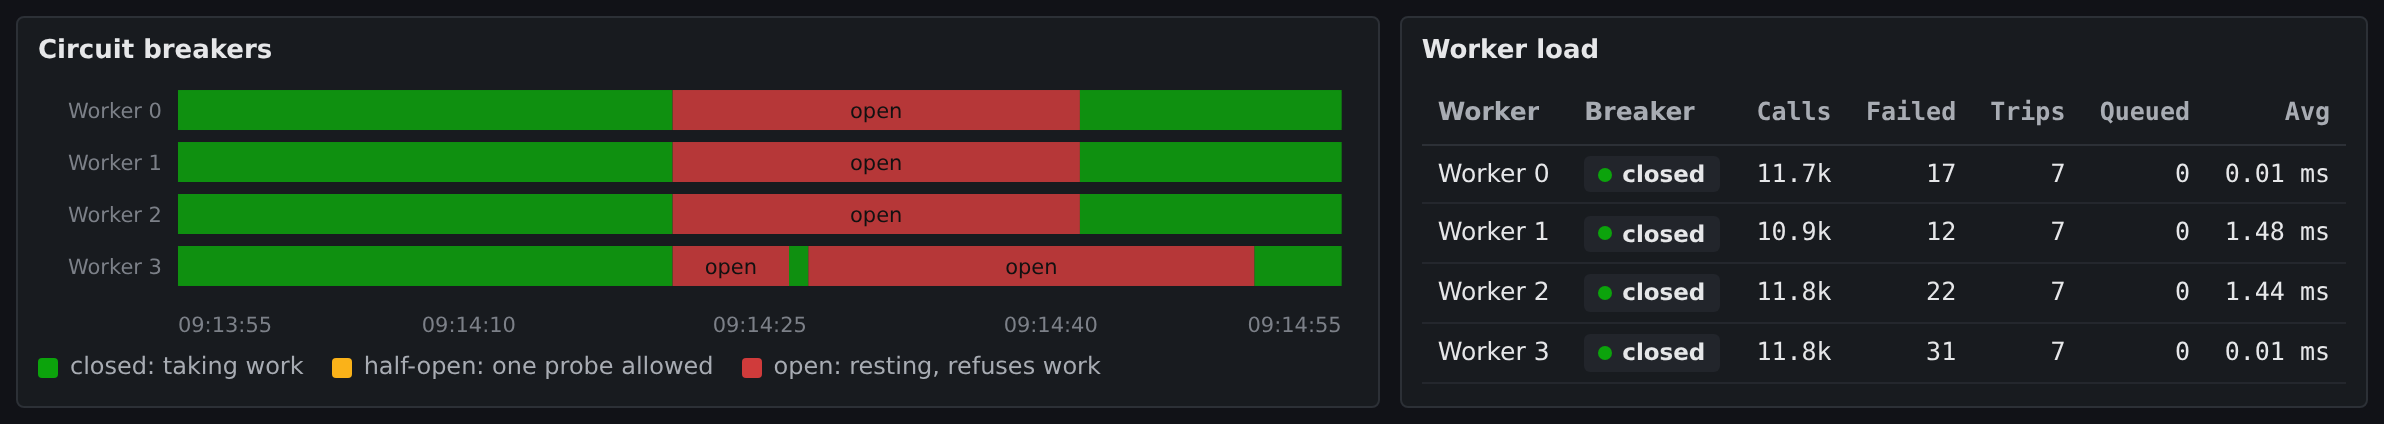
\includegraphics[width=\textwidth]{failures_recovered.png}
\caption{Failures test. Top: 60\% of lookups fail inside the workers; after 3 failures in a row each breaker
opens (red), so clients get a fast SERVFAIL. Bottom: with failures set back to 0\%, half-open probes succeed
and every breaker closes (green) without a restart.}
\label{fig:breakers}
\end{figure}

\begin{table}[H]
\centering\small
\caption{\code{load\_gen}: middleware alone, stub resolver ($\approx$5 ms), 8 client threads, 30\% duplicate names}\label{tab:load}
\begin{tabularx}{\textwidth}{@{}LrrrrP{3.2cm}@{}}
\toprule
Run & Queries & Throughput & SERVFAIL & Coalesced & Outcome \\
\midrule
Paced, 720 q/s (within capacity) & 20{,}000 & 720 q/s & 0 & 403 & p50 5 ms, p99 10 ms; exit 0 \\
Flood, unpaced & 100{,}000 & 59{,}851 q/s offered & 74{,}051 & 24{,}865 & overload shed in $\le$1 ms; every query 1 reply; exit 0 \\
Flood + 20\% resolver failures & 100{,}000 & 57{,}934 q/s offered & 75{,}913 & 24{,}727 & breakers tripped; exit 0 \\
1 worker, queue 1, 50 ms delay & 2{,}000 & --- & mostly overload & --- & exit 0 \\
\bottomrule
\end{tabularx}
\end{table}

\subsection{Security evaluation}
\begin{table}[H]
\centering\small
\caption{Security requirements against evidence}\label{tab:seceval}
\begin{tabularx}{\textwidth}{@{}lLP{2.0cm}@{}}
\toprule
Req. & Evidence and assessment & Verdict \\
\midrule
S1 & TLS 1.3 only (TLS 1.2 refused), X25519 ECDHE, AES-256-GCM. The capture has 0 decodable DNS frames and 0 occurrences of queried names. & Met \\
S2 & Lab: accepted only for the right name, CA and dates. Wrong name, expired, self-signed and wrong IP rejected live; untrusted, not-yet-valid and wildcard rejected in tests. Tests assert zero queries reach a rejected server, and a plain server is a failure, not a fallback. & Met \\
S3 & Client hop: three names of very different lengths all give 487 B replies. Upstream hop: every query 147 B and every answer 487 B, whatever the name, and even when the client asked for no padding. Before the fix for D4 the upstream records were 59--108 B and varied with the name. & Met \\
S4 & 123 wire-format tests plus live malformed messages: FORMERR or close, never a crash. Zero ASan/UBSan reports over the whole suite. & Met \\
S5 & Wrong-ID, wrong-question, garbage and junk-datagram tests; cache-only-own-chain test; bailiwick tests in recursion. & Met \\
S6 & Abusive client blocked in 0.09 s; polite client unaffected; flood answered exactly once per query; breakers open and close; every failure bounded by the deadline. & Met \\
S7 & Admin bound to 127.0.0.1; Host header checked (AdminServerTest). & Met \\
\bottomrule
\end{tabularx}
\end{table}

\textbf{What the evaluation does not show.}
\begin{itemize}
  \item The public-resolver path (Cloudflare, Google, Quad9) was exercised live only on a phone hotspot
  (Listing~\ref{lst:public}), not on the campus network, and not under the Traffic or Load tests: every unique
  name there would be a real query to a public resolver.
  \item Padding hides the reply's size, not its timing, nor the number of queries per page load.
  \item SNI on the upstream hop names the resolver being used, not the query.
\end{itemize}

\subsection{Defects discovered}\label{sec:defects}
\begin{tabularx}{\textwidth}{@{}lLP{2.4cm}@{}}
\toprule
ID & Defect & Status \\
\midrule
D1 & \code{DomainName} from wire: wrong size bound, two off-by-ones (next offset, compression pointer), missing overflow check before copying a label. Found by parser tests. & Fixed (6f7c47d) \\
D2 & Connection exhaustion: unsent answers exempted a connection from the idle timeout; trickled bytes counted as activity; no per-source connection cap. & Fixed (9825c9a), one test per fix \\
D3 & Flaky tests: per-test temp directories collided between processes; a fake-clock jump timed out a running lookup; a connect/reset race. & Fixed (9825c9a) \\
D4 & Queries to DoT upstreams carried no EDNS padding, so their size (59--108 B) leaked the name's length to an observer of the upstream hop. Found in this evaluation's capture. Fixed by padding every \code{tls://} query to 128 B, which also makes the upstream pad its answers. & Fixed (\code{Upstream}, \code{encode\_\allowbreak query}), 3 new tests \\
D5 & Dashboard sidebar clipped long ``Served by'' values: the grid cell lacked \code{min-width:0} and badges never wrapped. Found while taking this report's screenshots. & Fixed (\code{gui/\allowbreak index.html}) \\
D6 & Old sanitizer build directories configured with g++-14 fail to compile (\code{append\_range}). Build configuration only; fresh g++-15 configure passes. & Workaround: reconfigure \\
D7 & The final merge (f38d405) brought back \code{std::ranges::ends\_with} in \code{DomainName}, which GCC~15's standard library lacks, so \code{main} no longer compiled. Found when re-running the suite for this report. & Fixed (helper restored) \\
\bottomrule
\end{tabularx}

% =====================================================================
\section{Limitations and lessons learned}\label{sec:limits}

\subsection{Achieved requirements}
F1--F6 and S1--S7 are met; the one gap found during evaluation (upstream padding, D4) was fixed. Compared with the Stage~I plan we
added three things: an \emph{encrypted, certificate-checked upstream hop} (Stage~I listed it as a
non-goal), a full recursive resolver with zone files, and a live dashboard with built-in tests.

\subsection{Known weaknesses}
\begin{tabularx}{\textwidth}{@{}P{4.6cm}L@{}}
\toprule
Limitation & Effect \\
\midrule
Blocking resolvers & Cache-miss throughput $\approx$ workers $\times$ (1000 ms $\div$ upstream RTT): 100--150/s with 4 workers. Above that, queries get SERVFAIL ``expired in queue''. This is deliberate load shedding, but it limits capacity. \\
Cache checked inside the worker & Under overload, a cacheable query still waits behind slow lookups. \\
No negative caching & NXDOMAIN is asked upstream every time. \\
Query IDs from \code{mt19937} & Not cryptographically random; the random source port and TLS mitigate this. \\
No DNSSEC; recursion over IPv4 only & Answers are trusted as received; IPv6-only zones unreachable. \\
No certificate pinning & Any trusted CA's certificate for the name passes. \\
Rate limit per IP (IPv6 /64) & Clients behind one NAT share a bucket and a block (false positives). \\
\bottomrule
\end{tabularx}

\textbf{False positives and negatives.} The blocked-domain list matches exact names and their subdomains only.
A tracker on an unlisted domain passes (false negative), and blocking a parent blocks every child (possible
false positive). Abuse blocking can hit honest users behind a shared NAT. The thresholds (200 q/s, 50 strikes
in 10~s) are generous so that heavy browsing is never blocked: the ``Heavy, 250/s'' profile is rate-limited
but a polite 50/s client is never refused.

\textbf{Performance and usability.} Cached answers take 0.01--0.1~ms. Upstream DoT costs one extra round trip
only on a cold connection; afterwards 98\% of DoT queries rode a kept connection (2{,}283 of 2{,}339). The
dashboard explains every test in plain words and runs real traffic through the real middleware, which made the
evaluation reproducible. Its live log was the fastest way to see why a query failed.

\textbf{What the prototype does not guarantee.} It does not guarantee that answers are true (no DNSSEC), privacy
from the resolver operators, hiding of timing or traffic volume, or service beyond the configured capacity:
excess load is refused, not queued.

\subsection{Lessons learned}
\begin{itemize}
  \item \textbf{Narrow interfaces paid off.} Agreeing on \code{submit()} and \code{resolve()} in Stage~I let
  three people work in parallel against stubs and fakes. Integration took one day.
  \item \textbf{``Exactly once'' must be designed, not tested in.} Every way a query can end (answer, deadline,
  overload, exception, shutdown) goes through one atomic gate, and \code{load\_gen} exits non-zero if any
  query gets other than one reply.
  \item \textbf{Fail closed, fail fast.} A SERVFAIL in 1 ms beats a hung client. Bounded queues, deadlines and
  breakers turned every failure we injected into a quick, honest answer.
  \item \textbf{Test the network you will demo on.} The campus network blocks port 853 entirely. A local CA and
  a second instance let us test the real code path, the unreachable resolvers turned into timeout tests, and
  a phone hotspot confirmed the public resolvers work with the configuration unchanged.
  \item \textbf{Capture the wire.} The packet capture confirmed confidentiality and also found D4, which no unit
  test was looking for. After the fix, the same capture proved it closed.
\end{itemize}

\subsection{Five things to remember about this project}\label{sec:five}
\begin{tcolorbox}[breakable, enhanced jigsaw, colback=codebg, colframe=black!35, boxrule=0.4pt, arc=0pt, left=4pt, right=4pt, top=3pt, bottom=3pt]
\begin{enumerate}[leftmargin=*, itemsep=4pt]
  \item \textbf{Both hops are encrypted, and the transport is TLS over TCP.} Plain DNS on UDP port 53 lets
  anyone on the path read and forge every lookup. Clients reach the resolver with DNS-over-TLS (TCP 853), and
  the resolver uses DoT again to reach its upstream, so a query is never in clear text between the client and
  the server that answers it. TLS needs a reliable, ordered byte stream, which is why it runs over TCP rather
  than UDP. TLS~1.3 agrees a fresh key per connection with X25519 (forward secrecy) and encrypts with
  AES-256-GCM. The capture shows no readable DNS message and no queried name on either hop
  (Listing~\ref{lst:pcap}). The one exception is recursion, which must speak plain DNS to authoritative servers.
  \item \textbf{Encryption is only useful if you check who is on the other end, and you never fall back.} Before
  sending a question upstream, \code{TlsClient} requires the certificate to chain to a trusted CA, to match the
  configured name (or IP) and to be inside its validity dates. If a check fails, the next upstream is tried and
  then the client gets SERVFAIL. There is never a retry on plain port 53, so an attacker who blocks or
  intercepts port 853 gains nothing. The impostor, expired, self-signed and wrong-IP probes were all rejected
  with zero queries sent (Figure~\ref{fig:certs}).
  \item \textbf{Encryption hides the content but not the size, so messages are padded.} AES-GCM output is exactly
  as long as its input plus a 17-byte overhead, and a reply's length says a lot about the name. EDNS padding
  (RFC~7830/8467) rounds every message up to a fixed block: 468~B for replies when the client asks for padding,
  and 128~B for every query we send upstream. Every name then gives a 487~B reply record and a 147~B upstream
  query record. Padding is an EDNS option, so on the client hop the client decides; on the upstream hop we are
  the client, so we always pad. The capture is how we found that this was missing at first (D4).
  \item \textbf{Every query gets exactly one reply, and failure is fast.} An answer, the 2~s deadline, an
  overloaded queue, an exception and shutdown can all race to finish the same query. One atomic flag in the
  \code{Responder} lets exactly one of them reply. Bounded queues, a per-upstream time budget and per-worker
  circuit breakers turn every failure into a quick SERVFAIL instead of a client left waiting, and the service
  recovers on its own when the upstream returns. \code{load\_gen} checks the rule under a 100{,}000-query
  flood with injected failures (Table~\ref{tab:load}).
  \item \textbf{Untrusted input is rejected as early and as cheaply as possible.} A blocked source is reset
  before the TLS handshake, the most expensive work a client can cause. Connection caps (1000 in total, 32 per
  source), a token bucket per client and a strike count turn floods into REFUSED and then a 60~s block. Every
  read of client bytes is bounds-checked, so a lying length field, a compression loop or a 5-byte header ends
  in FORMERR or a closed connection, never a crash. The 128 wire-format tests ran clean under AddressSanitizer.
\end{enumerate}
\end{tcolorbox}

% =====================================================================
\section{Deployment and future work}

\subsection{Dependencies and build}
\needspace{10\baselineskip}
On Ubuntu:
\begin{lstlisting}[language=bash]
sudo add-apt-repository ppa:ubuntu-toolchain-r/test && sudo apt update
sudo apt install g++-15 cmake libssl-dev dnsutils         # CMake >= 3.21, OpenSSL 3
cmake --preset release && cmake --build --preset release  # dns_server, load_gen, dns_tests
\end{lstlisting}

\needspace{5\baselineskip}
On Fedora:
\begin{lstlisting}[language=bash]
sudo dnf install g++ cmake openssl-devel bind-utils       # CMake >= 3.21, OpenSSL 3
cmake --preset release && cmake --build --preset release  # dns_server, load_gen, dns_tests
\end{lstlisting}

\subsection{Run}
\begin{lstlisting}[language=bash]
./tools/make_demo_cert.sh                      # self-signed config/server.pem + .key (mode 600, git-ignored)
./build/release/dns_server config/demo.conf    # DoT on 127.0.0.1:8853, dashboard on http://127.0.0.1:8080/
dig +tls @127.0.0.1 -p 8853 example.com        # encrypted query
dig +tls @127.0.0.1 -p 8853 nas.lan            # local record
dig +tls @127.0.0.1 -p 8853 ad.doubleclick.net # REFUSED (blocked domain)
\end{lstlisting}
\needspace{8\baselineskip}
\code{config/demo.conf} forwards over DoT to \code{tls://1.1.1.1\#\allowbreak cloudflare-dns.com} and
\code{tls://8.8.8.8\#\allowbreak dns.google} using the system CA store. On a network that blocks port 853, pick a plain
resolver in the dashboard's resolver switch, or use a lab upstream as in Figure~\ref{fig:lab}:
\begin{lstlisting}
upstreams = tls://127.0.0.1:9853#resolver.lab.test
upstream_ca_file = /path/to/lab-ca.pem
\end{lstlisting}
For a real deployment: listen on \code{0.0.0.0:853} (needs \code{CAP\_NET\_BIND\_SERVICE}), use a CA-issued
certificate, and keep \code{admin\_listen} on loopback.

\subsection{Tests}
\begin{lstlisting}[language=bash]
ctest --test-dir build/release             # or ./build/release/dns_tests   (534 tests)
cmake --preset asan && cmake --build --preset asan && ctest --preset asan
cmake --preset tsan && cmake --build --preset tsan && ctest --preset tsan
./build/release/dns_tests --gtest_filter='DotUpstream*:TlsClient*:AdminTls*'   # upstream DoT evidence
./build/release/load_gen                   # exit 0 = every query got exactly one reply
./build/release/load_gen --stub-fail-rate 0.2
\end{lstlisting}

\subsection{Repository structure}
\begin{lstlisting}
include/            DomainName, IP, Records, dns_message (wire format), utils
include/mw/         middleware + front-end headers (namespace mw)
include/backend/    resolvers, Cache, Upstream / TlsClient
src/                library sources, main.cpp;  src/backend/  resolver sources
tests/              GoogleTest suite (31 files);  tests/support/  fake DNS / DoT servers, test CA, printers
tools/              load_gen.cpp, make_demo_cert.sh
gui/                index.html (dashboard, served by dns_server)
config/             demo.conf, demo.hosts, blocked_domains.txt, middleware.example.conf
docs/               frontend.md/.tex, this report
\end{lstlisting}

\subsection{Most important next improvements}
\begin{enumerate}
  \item \textbf{Asynchronous resolution}: one thread keeping many upstream queries open (epoll or io\_uring)
  and pipelining queries on a DoT connection (RFC 7766), so cache-miss throughput no longer scales with threads.
  \item \textbf{Check the cache in \code{submit()}} before queueing, so cached names are served even under
  overload; add negative caching (RFC 2308).
  \item \textbf{DNSSEC validation} in the recursive resolver, and optional SPKI pinning per upstream (RFC 7858
  \S4.2).
  \item \textbf{DoH front end} calling the same \code{submit()}, for clients and networks that allow only port
  443; cryptographic query IDs (\code{RAND\_bytes}); configuration reload on SIGHUP.
\end{enumerate}

% =====================================================================
\section{Appendix: minimum technical evidence index}

Project: \textbf{Encrypted DNS Resolver}. The chosen encrypted protocol is \textbf{DNS-over-TLS} (RFC 7858),
used on both the client hop and the upstream hop.

\begin{longtable}{@{}P{3.8cm}P{7.4cm}P{5.0cm}@{}}
\toprule
Required evidence & What is shown & Where \\
\midrule
\endhead
A DNS query completing through the encrypted protocol & \code{dig +tls} gets NOERROR; the dashboard shows it served by the upstream ``over TLS''; the capture shows only TLS 1.3 records on both hops, 0 DNS frames, no names, padded 487 B replies & Listing~\ref{lst:dig}, Figure~\ref{fig:lookup}, Listing~\ref{lst:pcap}, Figure~\ref{fig:overview} \\
\midrule
Client-side TLS parameters & TLS 1.3, AES-256-GCM, X25519; TLS 1.2 refused; key file mode 600, git-ignored & Section~\ref{sec:ev-dot} (\code{openssl s\_client}) \\
\midrule
Upstream certificate validation & Accepted certificate with subject, issuer, expiry, protocol; rejections for hostname mismatch, expired, self-signed, IP mismatch; ``nothing was asked''; counters and last-rejection reason; \code{openssl} cross-check & Figures~\ref{fig:certs}, \ref{fig:tlsrow}; Section~\ref{sec:ev-cert}; Table~\ref{tab:cases} \\
\midrule
Tests for invalid responses & Garbage, wrong ID or question, truncated, cut mid-frame, junk datagrams, malformed TCP; no poisoning of the next query; only own-chain records cached & Table~\ref{tab:cases}; \code{test\_dot\_upstream.cpp}, \code{test\_forwarding\_\allowbreak resolver.cpp} \\
\midrule
Tests for upstream failure & Closed port; upstream killed $\rightarrow$ fast SERVFAIL $\rightarrow$ recovery on restart; plain server where TLS expected (no fallback); next upstream tried after rejection; breakers open and close & Listing~\ref{lst:fail}, Figures~\ref{fig:log}, \ref{fig:breakers} \\
\midrule
Tests for timeouts & DoT upstream unreachable $\rightarrow$ SERVFAIL at 1000 ms; silent DoT server test; Compare test with all unreachable resolvers bounded & Listing~\ref{lst:fail}, Figures~\ref{fig:compare}, \ref{fig:log}; \code{SilentServerTimesOut} \\
\midrule
Malformed client input & FORMERR / NOTIMP / close for 12 hand-made messages & Listing~\ref{lst:neg} \\
\midrule
Availability & Abuse blocking, load results, exactly-once delivery & Figures~\ref{fig:abuse}, \ref{fig:overview}; Table~\ref{tab:load} \\
\midrule
Whole suite, sanitizers & 534/534 in release, ASan+UBSan, TSan & Table~\ref{tab:suite} \\
\bottomrule
\end{longtable}

\end{document}